%%%%%%%%%%%%%%%%%%%%%%%%%%%%%%%%%%%%%%%%
% PDF compatibility code. 
\makeatletter
\newif\ifpdflatex@
\ifx\pdftexversion\@undefined
\pdflatex@false
%\message{Not using pdf}
\else
\pdflatex@true
%\message{Using pdf}
\fi

\newcommand{\latexorpdf}[2]{
  \ifpdflatex@ #2
  \else #1
  \fi
}

\makeatother

\newcommand{\pformat}{a4paper}

%%%%%%%%%%%%%%%%%%%%%%%%%%%%%%%%%%%%%%%%

\latexorpdf{
\documentclass[\pformat,12pt]{jarticle}
}{
\documentclass[\pformat,pdftex,12pt]{jarticle}
}

\usepackage[dvipdfmx]{graphicx, color}
\usepackage[dvipdfmx,bookmarks=true,bookmarksnumbered=true,colorlinks,plainpages=true]{hyperref}

\usepackage{toolbox}
\usepackage{vdmsl-2e}
\usepackage{makeidx}
\usepackage{alltt}
%\usepackage{graphics}
%\usepackage{verbatim}
\usepackage{ifthen}
\usepackage{verbatimfiles}
%\usepackage{color}
\usepackage{longtable}
%\usepackage{path}
\usepackage{here}

\graphicspath{{figures/}}
\def\seename{$\Rightarrow$}

% Koizumi change start
\ifnum 42146=\euc"A4A2 \AtBeginDvi{\special{pdf:tounicode EUC-UCS2}}\else
\AtBeginDvi{\special{pdf:tounicode 90ms-RKSJ-UCS2}}\fi
% Koizumi change end

\makeindex

% The use of VDMSL/ ifdef's have basicly been exchanged with the
% use of LaTeX ifthenelse's.  For this two LaTeX boolean value VDMSL and
% VDMpp have been defined  (Lowercase p's are used to avoid conflict with
% the  environment variable.  The typical use are:
%   \ifthenelse{\boolean{VDMsl}}{vdmsl-text}{vdmpp-text}
%   \ifthenelse{\boolean{VDMsl}}{vdmsl-text}{}
%   \ifthenelse{\boolean{VDMpp}}{vdmpp-text}{}
% The advantage of this as opposed to ifdef's is that within a general
% paragraph specific VDM-SL and VDM++ parts can be distinguished without
% problematic empty lines.
% 
% The values are initialised such that exactly one of the values is true
% and the other is false.  This should hopefully avoid strange behaviour
% due to possible preprossing errors.  The default case is VDM-SL.
\newboolean{VDMsl}
\setboolean{VDMsl}{true}
\newboolean{VDMpp}
\setboolean{VDMpp}{false}
\setboolean{VDMpp}{true}
\setboolean{VDMsl}{false}


\def\vdmsl{{\small VDM-SL}}
\def\vdmpp{{\small VDM}$^{++}$}
\newcommand{\vdmslpp}{VDM++}
\newcommand{\vdmslppEm}{VDM\/++}
\newcommand{\ToolboxName}{VDM++ Toolbox}
\newcommand{\Toolbox}{Toolbox}
\newcommand{\toolbox}{toolbox}
\newcommand{\vdmde}{vppde}
\newcommand{\vdmgde}{vppgde}
\newcommand{\vdmhome}{vpphome}
\newcommand{\vdmdeNineteen}{vppde-19}
\newcommand{\vdmdeNineteenEl}{vppde-19.el}
\DeclareRobustCommand{\VdmSlPp}{VDM++-\VdmSl}

\newcommand{\guicmd}[1]{{\sf #1}}

\begin{document}
\vdmtoolsmanualscsk{C++コード生成マニュアル(VDM++)}{2.0}


\newcommand{\tcg}{コードジェネレータ}
\newcommand{\Tcg}{コードジェネレータ}

\newcommand{\libmancite}{\cite{LibMan-SCSK}}
\newcommand{\langmancite}{\cite{LangManPP-SCSK}}
%\newcommand{\VDM}{VDM\raisebox{-0.6ex}{++}}
\newcommand{\VDM}{VDM++}
\newcommand{\cg}{VDM++ to C++ コードジェネレータ}
%\newcommand{\toolbox}{VDM$^{++}$ Toolbox}
\newcommand{\MCL}{VDM C++ ライブラリ}
\newcommand{\CGBase}{\texttt{CGBase}}



%Installation should be described in the Installation document.
\section{導入}


\cg\ は、\VDM\ 仕様から C++ コード自動生成を行うための支援をする。
これにより、\tcg\ は \VDM\ 仕様に基づいたアプリケーションの実装を、速い方法で提供する。

 \Tcg\ は \ToolboxName{}に対しアドオン形式をとる。
このインストールについては、文書\ifthenelse{\boolean{VDMsl}}{\cite{InstallMan-SCSK}}{\cite{InstallPPMan-SCSK}}に記載されている。
本書は {\em VDMToolsユーザマニュアル( \VDM{} )}\ifthenelse{\boolean{VDMsl}}{\cite{UserMan-SCSK}}{\cite{UserManPP-SCSK}} の拡張であり、 \cg{}への導入を行う。

コードジェネレータは、 \VDM\ 構成要素全体のおよそ 95\% をサポートする。
補足として、 生成コードの一部を手書きコードに置き換えることがユーザーに許されている。

本書は以下のように構成されている:

第~\ref{invoking}章で、 \VDM\ 仕様が正しい C++ コードを生成するために満たされなければならない要件を並べる。
さらにこの章で、 \ToolboxName{}からC++ ファイルを起動する方法を述べる。
最後に、コード生成された C++ ファイルを記載する。

第~\ref{interfacing}章は、インターフェイスを記述しながら C++ 生成コードへの導入を行い、そしてそれをどのように手書きコードと結び付けるかを説明する。
さらに、 C++ コードのコンパイル、リンク、実行の方法まで説明する。

第~\ref{sec:unsupported}章では、 \tcg{}でサポートされない \VDM\ 構成要素をまとめて示す。

第~\ref{sec:relation}章は、C++ 生成コード構造の詳細を記載する。
加えて \VDM\ とC++ のデータ型間の関連を説明し、 \cg{}の開発中に用いる名称仕様を含めて、設計上決められている事柄をいくつか述べる。
ここは、\tcg\ を職業的に使用する前には集中的に学習すべき章である。


\section{コードジェネレータの起動}\label{invoking}


%Type \path+codegen+
%and the specification is type checked and the files \path+DefaultMod.h+
%and \path+DefaultMod.cc+ are generated (On Windows platforms the
%implementation file is named \path+DefaultMod.cpp+).

%A detailed description of the usage of the \cg{} is given in the
%Sections 4 and 5 in {\em User Manual for the IFAD \VDM{} Toolbox\/}
%\cite{UserMan}.
%#endif VDMSL

\tcg\ の使用を始めるため、1つ以上のファイルにわたった\VDM\ 仕様を書いておくべきであろう。
\Toolbox\ の配布中に、様々なソートアルゴリズムの仕様が含まれている。
この仕様は、以下において \tcg{}の使用を記述するために用いられることとなる。 
これは\ifthenelse{\boolean{VDMsl}}{\cite{SortEx-SCSK}}{\cite{SortExpp-SCSK}}で述べられている。
この手順1つ1つを、自身のコンピュータ上で確認していくことが推奨される。
そのため、ディレクトリ\path+vdmhome/examples/sort+ をコピーしそこへ \path+cd+ にて移動すること。

C++ コードを生成する前に、 \VDM\ 仕様が必要な要件を満たしているかどうか確認する必要がある。
この要件は第~\ref{requirements}章に記述されている。
第~\ref{gui} 章と ~\ref{commandline}章では、 \ToolboxName\ を用いてグラフィカルインターフェイスやコマンドラインから C++ コードを生成する方法を説明する。
第~\ref{sec:cppfiles}章では、コード生成された C++ ファイルを記載する。

\subsection{コード生成のための要件}\label{requirements}

 \Tcg\ が正しいコード生成を行うために、 \VDM\ 仕様の全ファイルは構文チェックされることが要件となる。
つまり1クラスのコード生成であっても、それを可能とするためには仕様中全ファイルのチェックが必要となる。

さらに \tcg\ は、適正な型のクラスに対してしかコード生成を行うことができない。
\footnote{ \langmancite で説明されるが、2つのよく形式化されたクラスが存在する。
ここではできるだけ十分によく形式化された型の適正さを意味する。} 
あるクラスに対して事前に型チェックを行わずコード生成しようとした場合は、 \Toolbox{}が自動的に型チェックを行う。 

\subsection{グラフィカルインターフェイスの利用}\label{gui}

ここでは \ToolboxName{}のグラフィカルユーザーインターフェイスから、どのようにソート例題をコード生成するかを述べていく。

\ToolboxName\ は\path+vdmgde+\index{vdmgde!starting}コマンドで始める。 
ソートの例題に相当するコードを生成するには、 \path+/vdmhome/examples/sort+ディレクトリに置かれたすべての\ifthenelse{\boolean{VDMpp}}{すべての {\tt *.rtf} ファイル}{ファイル {\tt  sort.rtf}} を含めて新しいプロジェクトを生成することである。
プロジェクトの構成法の記載としては、 \ifthenelse{\boolean{VDMsl}}{\cite{UserMan-SCSK}}{\cite{UserManPP-SCSK}} を参照のこと。

最初はファイルに対して構文チェックと型チェックを行う必要がある: 手作業で行わない場合には、\tcg\ が起動されるとき Toolbox が自動的にこれを行うはずである。
ソート例題の仕様では、エラーなしで両チェックを通過する。
その後\ifthenelse{\boolean{VDMsl}}{the module {\em DefaultMod}}{すべてのクラス} を選択して、\raisebox{-1.0mm}{
\includegraphics[width=0.03\textwidth]{cplusplus}} (\guicmd{Generate C++}) ボタンを押すことで、 \tcg\ が起動可能となる。
1つ以上のファイルあるいはクラスを選択することができ、この場合にはこれらが C++コードに翻訳される。
この手順の結果が 図~\ref{fig:cg}に示されている。


\begin{figure}[tbh]
\begin{center}
\mbox{}
\resizebox{9cm}{!}{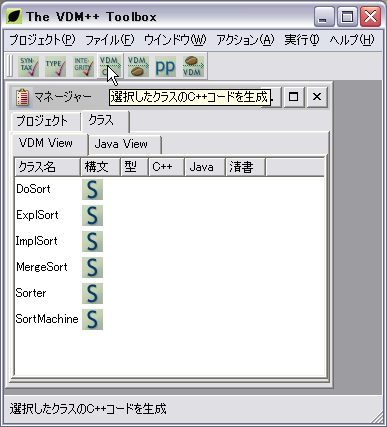
\includegraphics{cgpp1}}
\caption{ソート例題のコード生成}\label{fig:cg}
\end{center}
\end{figure}

仕様中の各 \ifthenelse{\boolean{VDMsl}}{module - in
  this example only one - }{クラス} に対してコードが生成されると、図~\ref{fig:cg2}に見られるようにToolbox は大きな {\em \large{C}}を書き入れてこれを知らせる。
プロジェクトファイルのおかれたディレクトリ中で、たくさんの C++ ファイルが生成される。
プロジェクトファイルの存在しない場合には、これらのファイルは \ToolboxName\ が始められたディレクトリに書かれることになる。

ソート例題に対してコード生成を行う時、\tcg{}によって警告が1つ生成されるため、図~\ref{fig:cg_error}のような {\em Error} ウィンドウが出る。

\begin{figure}[tbh]
\begin{center}
\mbox{}
\resizebox{9.2cm}{!}{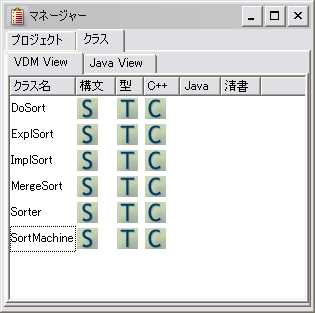
\includegraphics{cgpp2}}
\caption{ソート例題のコード生成}\label{fig:cg2}
\end{center}
\end{figure}


\begin{figure}[tbh]
\begin{center}
\mbox{}
\resizebox{9.2cm}{!}{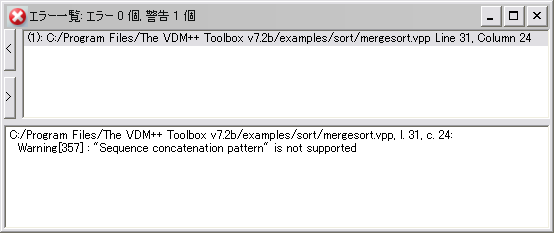
\includegraphics{cgpp3}}
\caption{コードジェネレータで生成された警告}\label{fig:cg_error}
\end{center}
\end{figure}


この警告は、\tcg{}では連結パターンがサポートされないことを示している。
\tcg\ はこの構成要素に対して、実行可能なC++ コード生成を行うことができないということを意味する。
生成されるコードはコンパイル可能なものであるが、サポートされない構成要素が含まれる枝葉部分の実行は実行時エラーを引き起こす。 
第~\ref{sec:unsupported}章で、サポートされない構成要素の詳細リストを提示する。

\tcg\ のユーザーは、実行時エラーの位置情報を含めたコード生成を選択できる。
{\em 出力位置情報} オプションが選択されていると、実行時エラーの原因である \VDM\ 仕様における位置 (ファイル名および行番号と列番号)を実行時エラーメッセージで伝えてくれる。
 図~\ref{fig:option}で示すように、オプションメニューでこの機能は設定できる。
もう1つ利用可能なオプションとして、 \textit{事前事後条件チェック}オプションがある。
これは、操作や関数の事前条件や関数の事後条件をチェックするコードを生成する。
これも図~\ref{fig:option}で示している。

\begin{figure}[tbh]
\begin{center}
\mbox{}
\resizebox{9cm}{!}{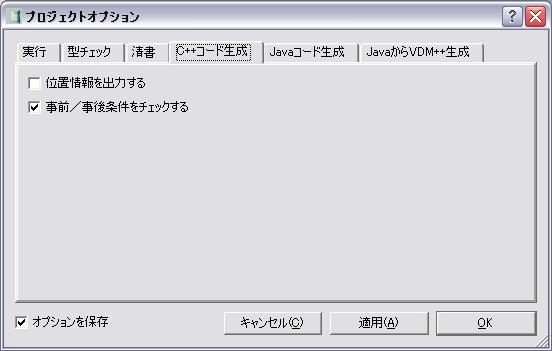
\includegraphics{cgpp4}}
\caption{C++ コードジェネレータのオプション}\label{fig:option}
\end{center}
\end{figure}
  
ソート例題に対しては \texttt{MergeSort} 関数の実行が、ここで述べた実行時エラーを引き起こす。
記載したオプション設定を行わなかった場合、相当する C++ コードの実行で次のエラーメッセージが出る:
\begin{quote}
\begin{verbatim}
The construct is not supported: Sequence concatenation pattern
\end{verbatim}
\end{quote}
一方、オプションを設定した場合は次のようなエラーメッセージとなる:
\begin{quote}
\begin{verbatim}
Last recorded position:
In: MergeSort. At line: 31 column: 18
The construct is not supported: Sequence concatenation pattern
\end{verbatim}
\end{quote}

\subsection{コマンドラインインターフェイスの使用}\label{commandline}

 \ToolboxName\ をコマンドラインから実行する場合にも、もちろん\Tcg\ を起動できる。
これは以下に簡単に述べられている。

\ToolboxName\ は、コマンドラインから {\tt  \vdmde}\index{vdmde!starting}コマンドで始める。コードを生成するために -c オプションを用いる:

\begin{quote}
\begin{verbatim}
vppde -c [-r] [-P] specfile, ...
\end{verbatim}
\end{quote}

ソート例題のコード生成を行うために、次のコマンドを
\path+vpphome/examples/sort+ ディレクトリで実行する:

\begin{quote}
\begin{verbatim}
vppde -c *.vpp
\end{verbatim}
\end{quote}

仕様は最初に構文解析がなされる。
構文エラーが検出されない場合、できる限り適正となるように型チェックがなされる。
型エラーが検出されなかった場合には、仕様は変換され最後にたくさんの C++ ファイルになる。
グラフィカルインターフェイスに相当するものとしては、実行時の位置情報をもつコード生成のために {\em  出力位置情報} オプション ({\tt -r}) を
設定することができ、さらに事前事後条件の実行時チェックを行うための \textit{事前事後条件チェック} オプション (\texttt{-P}) が設定できる。


\subsection{C++ 生成ファイル}\label{sec:cppfiles}

さらに1つ手順を進めて、コードジェネレータにより生成されたファイルを見てみよう。
\ifthenelse{\boolean{VDMsl}}{モジュール}{\VDM\ クラス}の各々に対して4つのファイルが生成される:

\begin{itemize}
\item \path+<ClassName>.h+
\item \path+<ClassName>.cc+
\item \path+<ClassName>_anonym.h+
\item \path+<ClassName>_anonym.cc+
\end{itemize}

 \path+<ClassName>.h+ ファイルは、 \VDM\ クラスに相当する C++ クラスの定義を含む。
さらに、 \VDM\ クラスで定義された合成型に相当するクラス定義を含む。

 \path+<ClassName>.cc+ ファイルは、 \VDM\ クラスで定義された関数と操作の実装を含む。
さらに、レコード型に対して生成される全クラスの要素関数の実装がここにある。

 \path+<ClassName>_anonym.h+ ファイルと \path+<ClassName>_anonym.cc+ ファイルは、全匿名型の宣言と実装を行うためにある。
匿名型とは、 \VDM\ 仕様において名前が与えられていないものである。

%When a class \path+M+ for example declares a type {\tt A =
%  set of int}, the \verb+M_anonym.h+ file will contain the declaration
%of a type \verb+type_iS+ and the \path+M.h+ file will contain a
%corresponding C++ \path+typedef+, as explained in the last section.

これらのファイルとは別に、さらに2つのファイルが生成される:
\begin{itemize}
\item \texttt{CGBase.h}
\item \texttt{CGBase.cc}
\end{itemize}

これらのファイルはオブジェクト参照型の一部の実装を含む。 
これは第~\ref{sec:classes}章で述べる。

%These files contains a class definition of {\em CGBase} which is super
%class to all non-derived classes. The {\em CGBase} class is part of
%modelling object reference of all instances of all the classes in the
%VDM++ specification that is generated. The {\em CGBase} class is
%described in Section~\ref{sec:classes}.
%
%The code corresponding to each \VDM{} class is divided into a header
%and an implementation file. Both files will be named with the class
%name. The suffix for the header file will be '.h', whereas the suffix
%for the implementation file will '.cc' on Unix platforms and '.cpp' on
%Windows platforms. The suffix of the implementation file can be
%customised by setting the environment variable {\bf
%VDMCGEXT}\footnote{On the Windows 95 platform this can be set in the
%\texttt{autoexec.bat} file, and on the Windows NT platform this can be
%set in the \texttt{Registry}}.


各 \VDM{} \ifthenelse{\boolean{VDMsl}}{module}{クラス}に相当するコードは、ヘッダーファイルと実装ファイルに分けられる。
両ファイルには \ifthenelse{\boolean{VDMsl}}{module}{クラス}名称が与えられる。
ヘッダーファイルの拡張子は '\texttt{.h}'となる一方、実装ファイルの拡張子は、Unixプラットフォーム上では '\texttt{.cc}' 、Windowプラットフォーム上では'\texttt{.cpp}' となる。
実装ファイルの拡張子は環境変数の設定により{\bf VDMCGEXT}\footnote{Windows 2000/XP/Vista上では \texttt{レジストリ}に設定できる}、カスタマイズすることができる。

\section{生成コードとのインターフェイス接続}\label{interfacing}

ここまでで、1つの\VDM\ 仕様からたくさんの C++ ファイルが生成されるところまで到達した。
アプリケーションのコンパイル・リンク・実行するためには、これらの C++ ファイルに対してインターフェイスを書くことになる。


生成コードに対しインターフェイスの記述を行うためには、生成コードについてのいくらか基本的な知識が必要となる。
これはまず、 \VDM\ 構成要素、特に \VDM\ 型に対してコード生成を行う時に、用いる方策を含める。
以下でこのことについて簡単な導入を行う。
さらなる情報は第~\ref{sec:relation}章に記載する。

\subsection{VDM++ 型のコード生成 - 基本}\label{basics}
この章では、\VDM\ の型をコード生成する方法について簡単な導入を行う。

まずは C++ 生成コードの例題を提示することから始める。
次は関数 \path+IsOrdered+のシグニチャである

\begin{quote}
\begin{verbatim}
IsOrdered: seq of int -> bool
\end{verbatim}
\end{quote}

\ifthenelse{\boolean{VDMsl}}{\path+DefaultMod+モジュールで定義されていて、}{\path+ExplSort+クラスで定義されていて、}
以下のようにコード生成される:

\begin{quote}
\begin{verbatim}
class type_iL : public SEQ<Int>{
...
};

Bool vdm_ExplSort::vdm_IsOrdered(const type_iL &vdm_l) {
...
};
\end{verbatim} 
\end{quote}

このコードを理解するため、 VDM 型に対してコード生成を行うための方策を知ると共に、同様に用いられる名称仕様についても、いくらか知識が必要となる。

 \tcg{} のデータ型の扱いは、 \MCL{}に基づく。 
このライブラリ (\path+libvdm.a+) の最新版を \libmancite に記載する。

\begin{itemize}

\item {\em 基本データ型}

基本データ型は、相当する VDM C++ ライブラリクラスである、 \path+Bool+、 \path+Int+、 {\tt    Real}、 \path+Char+ 、 \path+Token+にマップされる。

\item {\em 引用型}

  引用型は、相当する VDM C++ ライブラリクラス {\tt Quote}にマップされる。

\item {\em 集合、列、写像型}
  
合成型 \path+set+、 \path+sequence+ 、 \path+map+、を取り扱うために、テンプレートが導入されている。
これらテンプレートは VDM C++ ライブラリにおいても定義されている。
例として、VDM 型である \verb+seq of int+ がどのようにコード生成されるかを見よう:\begin{quote}
\begin{verbatim}
class type_iL : public SEQ<Int>{
...
};
\end{verbatim}
\end{quote}

   VDM \path+seq+ 型は、テンプレートである \path+SEQ+ クラスから継承されるクラスにマップされる。
\verb+seq of int+の場合、テンプレートクラスの引数は \path+Int+であり、これは基本的な VDM 型 \path+int+を表す C++ クラスである。
新しいクラスの名称は以下のように作られている:

\begin{quote}
\verb+type+ : 匿名型を示す\\
\verb+i+: 整数を示す\\
\verb+L+: 列を示す\\
\end{quote}

\item {\em 合成型/レコード型}
  
  各合成型はマップされて、 VDM C++ ライブラリ \path+Record+ クラスのサブクラスにマップされる。
たとえば次の \ifthenelse{\boolean{VDMsl}}{モジュール \path+M+で}{クラス \path+M+で}定義された次の合成型は
\begin{quote}
\begin{verbatim}
A:: r : real
    i : int
\end{verbatim}
\end{quote}
以下のようにコード生成される:
\begin{quote}
\begin{verbatim}
class TYPE_M_A : public Record{
...
};
\end{verbatim}
\end{quote}

\item {\em 組型}

組の取り扱いは、合成型に対するものと大変よく似ている。
各組型は、VDM C++ ライブラリ \path+Tuple+ クラスのサブクラスにマップされる。
たとえば、次の組は:
\begin{quote}
\begin{verbatim}
int * real
\end{verbatim}
\end{quote}
以下のようにコード生成される:
\begin{quote}
\begin{verbatim}
class type_ir2P : public Tuple{
...
};
\end{verbatim}
\end{quote}

新しいクラス名称は次の方法で作成される:

\begin{quote}
\verb+type+ : 匿名型を示す\\
\verb+i+: 整数を示す\\
\verb+r+: 実数を示す\\
\verb+2P+: 次数2の組を示す\\
\end{quote}

\item {\em ユニオン型}

ユニオン型は、VDM C++ ライブラリ \path+Generic+ クラスにマップされる。

\item {\em オプション型}

オプション型はマップされ VDM  C++ ライブラリの \path+Generic+ クラスとなる。


\item {\em オブジェクト参照型}

各 VDM++ クラスに対して相当する C++ クラスが生成される。
VDM++クラス {\em SortMachine} に対しては、相当する C++ クラス {\em
  vdm\_SortMachine} が生成される。

クラスインスタンスのオブジェクト参照は、クラス\path+type_ref_<ClassName>+にマップされる。

オブジェクト参照型のことは第~\ref{sec:classes}章で詳細に述べる。 

\end{itemize}


合成型の例において、既に型名称の生成方法について構想が与えられている。

仕様において名称が与えられていない型(匿名型)には、小文字の \path+type+ が前につけられる。
しかし型名称には大文字で \path+TYPE+ が前に付けられる。
既にレコード例題で、 {\tt  TYPE\_M\_A}と名づけられた型名称の例を見てきた。
他の \VDM\ 型ももちろん名付けることができ、名称スキームはレコード型に対して用いたのと同じである。

生成される型名称には、 \path+TYPE+が前に付けられる。
その後 \ifthenelse{\boolean{VDMsl}}{モジュール名}{クラス名}が続き、ここで型が定義され、最後に選択されたVDM 名称が連結される。

以下の \VDM\ 仕様と定義型の生成では、用いられた名称仕様を見よう:

\begin{quote}
\begin{verbatim}
class M
types
  A = int;
  B = int * real;
  C = seq of int;
end M
\end{verbatim}
\end{quote}

上記3つの定義型には、名称 \verb+TYPE_M_A+、\verb+TYPE_M_B+ 、 \verb+TYPE_M_C+が与えられる。
これら型名称のスコープは \ifthenelse{\boolean{VDMpp}}{クラス}{モジュール}\ \path+M+に限定される。
したがってこれらの名称定義は、ファイル {\em  M.h}に置かれる。 

\begin{verbatim}
 #define TYPE_M_A Int 
 #define TYPE_M_B type_ir2P 
 #define TYPE_M_C type_iL
\end{verbatim}


しかし、仕様はまた2つの匿名型 {\tt  int * real} と \verb+seq of int+も含める。
これらの型は潜在的にどのような \ifthenelse{\boolean{VDMpp}}{クラス}{モジュール}でも用いることができ、したがって相当する C++ 型の名称と定義はグローバルに\footnote{構造的に等しい型に対して単一の名称を定義するという方策である。
この方策は C++ は型名称等価に基づくという現実に対処するために用いられ、一方で VDM++ は構造等価に基づいている。 }宣言および定義されるべきである。
これは{\em anonym} ファイル内でなされている: 
\path+<ClassName>_anonym.{h,cc}+


型がコード生成される方法について与えられる情報に加え、どのように関数や操作の名称が生成されるかについて触れておくべきだ:  VDM 仕様内の  M \ifthenelse{\boolean{VDMsl}}{モジュール}{クラス}における関数あるいは操作の名称 \path+f+ に対し、次の名称が与えられる:
\path+vdm_M::vdm_f+.

ここでVDM 仕様に対してコード生成を行う際の \tcg{} の全体的方策を把握しておくべきであろう。
さらに詳細な情報は第~\ref{sec:relation}章で述べるので、 \tcg\ を専門的に用いる場合は丁寧に学習する必要がある。

\subsection{ユーザーにより実装されたファイル}

 \tcg\ およびコード生成されたファイルについて、基本的な情報はここまでですでに述べた。
この章では、生成コードとインターフェイスをとるために行わなければならない作業を述べる。

まず、\VDM\ 仕様に対するC++コードを実行する場合に含まれるすべての C++ ファイルについて、概観を示すことから始めよう。
これらのファイルは、コード生成される C++ ファイルと手作業でコーディングされる C++ ファイルに分けることができる。
図~\ref{fig:cppfiles} では、コード生成ファイルを左に、手書きファイルを右に示している。
さらにそれらに含まれるファイルを、\VDM\ \ifthenelse{\boolean{VDMsl}}{モジュール}{クラス} 単位の C++ ファイルと \VDM\ 仕様単位の C++ ファイルに分けることができる。

\begin{figure}[tbh]
\begin{center}
\begin{picture}(400,300)(0,0)
\put(0,0){\framebox(150,70)[c]{%
  \parbox{4.5cm}{
  \texttt{<Classname>.h}
  \texttt{<Classname>.cc}
  \texttt{<Classname>\_anonym.h}
  \texttt{<Classname>\_anonym.cc}
  }
}}

\put(250,0){\framebox(150,70)[c]{
  \parbox{5cm}{
  \texttt{<Classname>\_userdef.h}
  \texttt{<Classname>\_userimpl.cc}
  }
}}

\put(0,230){\framebox(150,70)[c]{
  \parbox{4.5cm}{
    \texttt{CGBase.h}
    \texttt{CGBase.cc}
  }
}}

\put(250,230){\framebox(150,70)[c]{
  \parbox{4.5cm}{
    メインプログラム
  }
}}

\put(125,115){\framebox(150,70)[c]{
  \parbox{4.5cm}{
    \VDM\ 仕様/ プロジェクト
  }
}}

\put(125,115){\vector(-1,-1){44}}
\put(275,115){\vector(1,-1){44}}
\put(125,185){\vector(-1,1){44}}
\put(275,185){\vector(1,1){44}}

\put(200,35){\makebox(0,0){\parbox{2.4cm}{%
  \raggedright \VDM\ 
    \ifthenelse{\boolean{VDMsl}}{モジュール}{クラス}
  単位 C++ ファイル
  }
}
}

\put(200,265){\makebox(0,0){\parbox{2.4cm}{%
\raggedright \VDM\ プロジェクト毎の\VDM\ C++ ファイル}
}}

\put(75,150){\makebox(0,0){\parbox{2.4cm}{%
\raggedright コード生成 C++ ファイル}}}

\put(325,150){\makebox(0,0){\parbox{2.4cm}{%
\raggedright 手書き C++ ファイル}}}

\end{picture}


\caption{\VDM\ プロジェクト単位のC++ファイル}\label{fig:cppfiles}
\end{center}
\end{figure}

第~\ref{sec:cppfiles}章ですでに、コード生成された C++ ファイルについて述べた。
ここでは手書きコードファイルについて述べよう。

生成コードとインターフェイスをとるために、以下の作業の完了が必要である:

\begin{enumerate}
\item 各 \ifthenelse{\boolean{VDMsl}}{モジュール}{クラス}に対して、レコードタグに用いるオフセットを定義する。
\item  \VDM\ 仕様に含まれている陰関数/陰操作および宣言文を実装する。
\item メインプログラムを書く。
\item 選択的に、生成された C++ コードを部分的に手書きコードと置き換える。
\item アプリケーションのコンパイル、リンク、実行を行う。
\end{enumerate}

以下ではソート例題について、これらの作業を順に1つ1つ説明していく。

\subsubsection{レコードタグに用いるオフセットの定義}

 \VDM\ 仕様において合成型(レコード型)は、文字列(タグ)とレコード型の各項目に対する選択項目の並びで構成される:

\begin{quote}
\begin{verbatim}
RecTag ::
  fieldsel1 : nat
  fieldsel2 : bool
\end{verbatim}
\end{quote}

VDM C++ ライブラリでは、レコードタグ文字列 {\em ``RecTag''} が単一整数を用いてモデル化されている。
しかしこの方策をとるためには、1つの仕様に含まれる全レコード型が各々単一のタグ番号を有していることが重要である。
 \tcg\ は各\ifthenelse{\boolean{VDMpp}}{クラス}{モジュール}\ に対し、オフセットを基として連続的にレコードタグ番号を振り当てる。
オフセットはユーザーによって定義されるべきものであり、各 \ifthenelse{\boolean{VDMpp}}{クラス}{モジュール}\ に対し定義されるオフセットがタグの唯一性を保証するものとなるかどうかは、ユーザーの責任である。

オフセット定義は、
\path+<ClassName>_userdef.h+
という名のファイル中に書き込まれるべきである。
%\ifthenelse{\boolean{VDMsl}}{\path+<ModuleName>_userdef.h+}
%{\path+<ClassName>_userdef.h+}. 
オフセットは定義命令で定義し、
タグは
\path+TAG_<ClassName>+.
%\ifthenelse{\boolean{VDMpp}}{\path+TAG_<ClassName>+}{\path+TAG_<ModuleName>+}.
という名称とするべきである。

ソート例題においてユーザーは、各クラスに1つで6つのファイルを実装する必要がある。
 \verb+MergeSort_userdef.h+ ファイルには、たとえば次のような定義が含まれるだろう。

\begin{verbatim}
 #define TAG_MergeSort 100
\end{verbatim}


\subsubsection{陰関数/陰操作および宣言文の実装}\label{implicit}

陰関数を含むすべての \ifthenelse{\boolean{VDMsl}}{モジュール}{クラス} に対して、その関数定義を含んだ
\path+<ClassName>_userimpl.cc+
%\ifthenelse{\boolean{VDMsl}}{\path+<ModuleName>_userimpl.cc+}{\path+<ClassName>_userimpl.cc+}
というファイルが書かれる必要がある。


ソート例題は \path+ImplSort+クラス内に、\path+ImplSorter+という陰関数を1つ含む。
生成されたC++コードのインターフェイスのために、この関数は \path+ImplSort_userimpl.cc+ ファイル中に実装されていなければならない。
この関数は \path+ImplSort.h+ファイル中に定義されているもので、 \path+vdm_ImplSort+クラス中に見つかるその要素関数宣言と一致するように書かれていなければならない:

\begin{quote}
\begin{verbatim}
virtual type_iL vdm_ImplSorter(const type_iL &);
\end{verbatim}
\end{quote}

クラス \path+ImplSort+ 中の関数 \path+ImplSorter+ は\path+vdm_ImplSort::vdm_ImplSorter+ という名称となり、以下のように宣言される:

\begin{quote}
\begin{verbatim}
type_iL vdm_ImplSort::vdm_ImplSorter(const type_iL& l) {
...
}
\end{verbatim}
\end{quote}

この関数の実装の一例を 付録 \ref{sec:implsort}に示してある。


このようにユーザーは、操作に対して C++ 関数定義を書き、それを含む \ifthenelse{\boolean{VDMsl}}{モジュール}{クラス}を
\path+<ClassName>_userimpl.cc+
ファイルに加えなければならない。


コードジェネレータは、出会った宣言文の各々に対しインクルード命令を作成する。
このようにユーザーは、各仕様文に対して相当する名称のファイル: 
\path+vdm_<ClassName>_<OperationName>-<No>.cc+, 
を実装する必要があるが、
ここにおける\path+<OperationName>+ は宣言文が現れる操作の名称で、\path+<No>+ は操作仕様にある仕様文に連続番号をふったものとなる。



\subsubsection{メインプログラムの実装}
ここまで、メインプログラムを除くコードのコンパイル、リンク、実行に必要なファイルの実装を行ってきた。

ここで、ソート例題に対するメインプログラムを書いてみよう。

まず、\VDM{}のメインプログラムの仕様を定めることから始めることとする。

\begin{quote}
\begin{verbatim}
01   Main: () ==> ()
02   Main () ==
03     let arr1 = [3,5,2,23,1,42,98,31],
04         arr2 = [3,1,2] in
05  
06     ( dcl smach : SortMachine := new SortMachine(),
07           res : seq of int = [];
08       def dos : Sorter := new DoSort() in
09       res = smach.SetAndSort(dos,arr1);
10       def expls : Sorter := new ExplSort() in
11       res = smach.SetAndSort(expls,arr2);
12       def imps  : Sorter := new ImplSort() in
13       ( res = smach.SetAndSort(imps,arr2)
14         imps.Post_ImplSorter(arr2,res)
15       )
16      def mergs : Sorter := new MergeSort() in
17       smach.SetSort(mergs);
18      res = smach.GoSorting(arr2);
19     )
\end{verbatim}
\end{quote}

そして上記仕様の、 \VDM\ メソッドと同等の機能を有するC++のメインプログラムを実装していく。
メインプログラムは \path+sort_pp.cc+ に実装されていて、全プログラムを 付録 \ref{sec:main}で見ることができる。

メインプログラムを含めた C++ ファイルは、すべての必要なヘッダーファイルをすべてインクルードすることから始めるべきである。
これらは、各 \VDM\ クラスごとのヘッダー、\MCL{} のヘッダー、\path+metaiv.h+、そして(出力を生成するための)標準ライブラリクラス\path+<fstream>+ を含める。

ここでは、上記に列挙した VDM 仕様を順次 C++へ翻訳していこう。
%\footnote{One could also code generate the listed \VDM\ 
%  specification and then write a main program calling the generated
%  \path+vdm_Main+ function. However, this would not be very helpful in
%  learning something about the way to interface with the generated
%  code. Moreover, it would not be possible to generate some output.}
%
行 \path+03+ と \path+04+ で2つの整数リストが明記される。
 C++に翻訳されると次のコードとなる:
\begin{quote}
\begin{verbatim}
type_iL arr1, arr2;
arr1.ImpAppend ((Int)3);
arr1.ImpAppend ((Int)5);
...
arr2.ImpAppend ((Int)3).ImpAppend ((Int)1).ImpAppend ((Int)2);
\end{verbatim}
\end{quote}

行 \path+06+ は、 \path+SortMachine+クラスのインスタンスに対するオブジェクト参照 \path+smach+ を宣言している。

次の行はこれをC++で実装する:
\begin{quote}
\begin{verbatim}
type_ref_SortMachine smach (ObjectRef (new vdm_SortMachine ()));
\end{verbatim}
\end{quote}

行 \path+07+ は  \verb+seq of int+ 型の変数 \path+res+ を宣言していて、これは後にソートされた整数列を含めるために用いられる。
これに対するC++ コードは次の通り:

\begin{quote}
\begin{verbatim}
type_iL res;
\end{verbatim}
\end{quote}

ここでどのようにして仕様のソートメソッドを呼び出すかを見よう。

 \VDM\ 仕様と生成された C++コードから分かるように、 \path+SortMachine+ クラスはインスタンス変数として\path+Sorter+ 抽象型クラスに対するオブジェクト参照をもつ。
 \path+Sorter+ のサブクラスは異なるソートアルゴリズムを実装している。
 \path+SortMachine+ クラスの \path+SetAndSort+ メソッドは2つのパラメータをもつ:\path+Sorter+ のサブクラスのインスタンスと整数の列である。
メソッドは、前述のインスタンス変数が特定のサブクラスしたがって特定のソートアルゴリズムを参照するように設定し、その後このクラスの \path+Sort+ メソッドを整数列をパラメータとして呼び出す。
結果はソート済みの整数列となるはずである。

行 \path+08+ は、 \path+DoSort+クラスのインスタンスに対するオブジェクト参照 \path+dos+ を宣言し、 \path+SortMachine+ クラスの \path+SetAndSort+メソッドを宣言されたオブジェクト参照 \path+dos+ と整数列 \path+arr1+ を引数として呼び出す。
結果は \path+res+で与えられる。

すべてのコード生成された \VDM\ 型は \path+ascii+ メソッドをもち、それぞれのVDM 値の ASCII 表現を含んでいる文字列を返す。
このメソッドは、ここでは関連するログメッセージを実行中に標準出力にプリントするために用いられている。
{\tt  SortMachine} クラスに対する参照は、コード生成されたクラス {\tt CGBase}で定義された\verb+ObjGet_vdm_SortMachine+ 関数を呼び出すことで得られる。

\begin{quote}
\begin{verbatim}
cout << "Evaluating DoSort(" << arr1.ascii () << "):\n";
type_ref_Sorter dos (ObjectRef (new vdm_DoSort ()));
res = ObjGet_vdm_SortMachine(smach)->
        vdm_SetAndSort (dos, arr1);
cout << res.ascii() << "\n\n";
\end{verbatim}  
\end{quote}

 \path+ExplSort+クラスで定義されたソートアルゴリズムで \path+arr2+ をソートするため、同じような次のコードが書ける:
\begin{quote}
\begin{verbatim}
cout << "Evaluating ExplSort(" << arr2.ascii () << "):\n";
type_ref_Sorter expls (ObjectRef(new vdm_ExplSort ()));
res = ObjGet_vdm_SortMachine(smach)->
        vdm_SetAndSort (expls, arr2);
cout << res.ascii() << "\n\n";
\end{verbatim}
\end{quote}

 \path+ImplSort+クラスで実装されたソートアルゴリズムで \path+arr2+ をソートするため、次のコードが書ける:
\begin{quote}
\begin{verbatim}
cout << "Evaluating ImplSort(" << arr2.ascii () << "):\n";
type_ref_Sorter imps (ObjectRef(new vdm_ImplSort ()));
res = ObjGet_vdm_SortMachine(smach)->
        vdm_SetAndSort (imps, arr2);
cout << res.ascii() << "\n\n";
\end{verbatim}
\end{quote}
注意したいのは、コードに対するインターフェイスは陰や陽の関数/操作をもつことに依存しないということだ。

同様に、 \path+ImplSort+に対して事後条件関数を呼び出したい場合を想定できるだろう。
これに対して\Tcg\ は \path+vdm_ImplSort+ クラス内に\path+vdm_post_ImplSorter+ という名称の関数を生成した。
これは通常の方法で呼び出すことができる。
\begin{quote}
\begin{verbatim}
cout << "Evaluating post condition for ImplSort:\n";
Bool p = ObjGet_vdm_ImplSort(imps)->
           vdm_post_ImplSorter (arr2, res);
cout << "post_ImplSort(" << arr2.ascii () << "," <<
  res.ascii () <<  "):\n" << p.ascii () << "\n\n";
\end{verbatim}
\end{quote}

{\tt  SortMachine}クラスの \path+SetAndSort+ メソッドを呼び出す代わりに、16行から18行目で示すように最初は \path+SetSort+ を呼び出すことで、求めるソートアルゴリズムの設定を選択できる。
ここでは \path+MergeSort+ アルゴリズムを選択するが、結果のC++ コードに実行時エラーが含まれてしまうことが知られている。
結果のコードを次に示す:

\begin{quote}
\begin{verbatim}
type_ref_Sorter mergs (ObjectRef(new vdm_MergeSort ()));
ObjGet_vdm_SortMachine(smach)->vdm_SetSort (mergs);

cout << "Evaluating MergeSort(" << arr2.ascii () << "):\n";
res = ObjGet_vdm_SortMachine(smach)->vdm_GoSorting(arr2);
cout << res.ascii() << "\n\n";
\end{verbatim}  
\end{quote}


%?? The \MCL{} is implemented in a way such that compound types can
%?? contain elements of any VDM type (\path+Generic+). This means that an
%?? object of any VDM C++ class can automatically be casted to a {\tt
%??   Generic}. For example, the \VDM{} type \path+seq of nat+ is
%?? translated into a \path+Sequence+ in the generated code.
%??

記述のメインプログラムは\path+sort_pp.cc+ という名称のファイルに実装され、これは付録 \ref{sec:main}に一覧されている。 



\subsubsection{生成された C++ コードの部分的置き換え}\label{substituting}


最後に、生成された C++ コードを手書きコードへ置き換える可能性についていくつか述べておくべきだ。
これが役に立つ状況として、主な2つを挙げることができる:

\begin{itemize}
\item  \tcg{}でサポートされない構成要素に対してコード実装を行いたい場合。
\item 今ある構成要素をより効果的に実装したい場合。
\end{itemize}

ソート例題に関して、 \ifthenelse{\boolean{VDMsl}}{{\tt  MergeSort}}{\path+MergeSorter+} 関数の手書きコード版を実装したいという場合が想定されるが、そこに \tcg{}でサポートされていない構成要素が含まれているからである。
そのためコード生成された関数
\path+vdm_MergeSort::vdm_MergeSorter+
を手書き版に置き換えることが、ユーザーにとっては必要となる。 
そのためには新しい関数を書く必要がある。
これは 
\path+MergeSort.cc+:
の生成コード版と同じ宣言ヘッダーをもたなければならない。

\begin{quote}
\begin{verbatim}
type_rL vdm_MergeSort::vdm_MergeSorter(const type_rL &vdm_l) {
...
}
\end{verbatim}
\end{quote}

生成コード関数を手書き関数と置き換えるために、この関数は
\path+MergeSort_userimpl.cc+
という名のファイルに実装される必要があり、さらに以下の2つの定義が
\path+MergeSort_userdef.h+
ファイルに追加される必要がある:


\begin{quote}
\begin{verbatim}
 #define DEF_MergeSort_USERIMPL    
   // a user defined file is now included.Note: For classes
   // containing implicit functions/operations, an user
   // implemented file is a presumption and this line should be
   // obmitted.
 #define DEF_MergeSort_MergeSorter 
   //  the MergeSorter function in class MergeSort is handcoded 
\end{verbatim}
\end{quote}


このように \tcg\ で生成された特定の関数は手書き関数に置き換えることができる。

\subsection{C++コードのコンパイル、リンク、実行}
ユーザーが前に述べたファイルの手書きを行った場合、その後はC++コードのコンパイル、リンク、実行を行うこととなる。

 \cg{} のこの版で生成されたC++ コードは、以下のサポート対象コンパイラを用いてコンパイルされなければならない:

\begin{itemize}
\item Microsoft Windows 2000/XP/Vista上のMicrosoft Visual C++ 2005 SP1
\item Mac OS X 10.4, 10.5
\item Linux Kernel 2.4, 2.6上のGNU gcc 3, 4
\item Solaris 10
\end{itemize}

 \cg{} のこの版で生成されたC++ コードは、以下のサポート対象コンパイラを用いてコンパイルされなければならない:

\begin{itemize}
\item \path+libCG.a+: コード生成補助関数。このライブラリは \cg{} と共にリリースされたもので、付録 \ref{sec:libCG}に記載されている。
\item \path+libvdm.a+: \MCL{}。このライブラリは \cg{} と共にリリースされたもので、\libmancite に記載されている。
\item \path+libm.a+: コンパイラ対応の数学ライブラリ。
\end{itemize}



ソート例題の実装で用いられる \path+Makefile+ は付録 \ref{sec:make}に一覧されている。 
メインプログラム \path+sort_pp+をコンパイルするために、 \path+make+ \path+sort_pp+とタイプする必要がある。

% Note that all the classes in the example are code generated in advance.



ここまでくれば、メインプログラム \path+sort_pp+の実行が可能になる。
結果は以下にリストされている。
 \path+MergeSort+の実行中に実行時エラーがおきてしまうことには注意しよう。
これは、サポートされていない構成要素を実行しようとした場合に引き起こされる。
生成コードに含まれている位置情報が、基礎を成す仕様におけるエラーを導く。

\begin{quote}
\begin{verbatim}
$  sort_pp
Evaluating DoSort([ 3,5,2,23,1,42,98,31 ]):
[ 1,2,3,5,23,31,42,98 ]

Evaluating ExplSort([ 3,1,2 ]):
[ 1,2,3 ]

Evaluating ImplSort([ 3,1,2 ]):
[ 1,2,3 ]

Evaluating post condition for ImplSort:
post_ImplSort([ 3,1,2 ],[ 1,2,3 ]):
true

Evaluating MergeSort([ 3,1,2 ]):
Last recorded position:
In: MergeSort. At line: 26 column: 18
The construct is not supported: Sequence concatenation pattern
$
\end{verbatim}
\end{quote}


\section{サポートされていない構成要素}\label{sec:unsupported}

 この版の\tcg\ では以下の \VDM\ 構成要素はサポートされていない:

\begin{itemize}

%% Is not part of the language manual any longer!
%\item The Real-time part of \VDM{}. 
\item 式:

  \begin{itemize}
  \item ラムダ式。
  \item 合成式、繰り返し式、関数の同値式。
  \item 関数型インスタンス化式。ただし以下の例題にあるように、コードジェネレータは適用式と組み合わせて関数型インスタンス化式をサポートする:

\begin{quote}
\begin{verbatim}
Test:() -> set of int
Test() ==
  ElemToSet[int](-1);

ElemToSet[@elem]: @elem +> set of @elem
ElemToSet(e) ==
  {e}
\end{verbatim}
\end{quote}

\item  \VDM{}の同時平行性の部分で、 {\tt \#act}、 {\tt \#fin} {\tt \#active}、 {\tt \#waiting} 、 {\tt \#req}の式。

  \end{itemize}

\item 文: 

  \begin{itemize}
  \item always文、exit文、 trap文、recursive trap 文。
  \item start文と start list 文。
  \end{itemize}

\item 次における型束縛 (\langmancite 参照):

  \begin{itemize}
  \item let-be-st 式/文。
  \item 列、集合、写像の包含式。
  \item iota 式と量化式。
  \end{itemize}

例題として次の式は \tcg によってサポートされている:


\begin{quote}
\begin{verbatim}
let x in set numbers in x
\end{verbatim}
\end{quote}

一方、次はサポートされていない (原因は型束縛 \verb+n: nat+):

\begin{quote}
\begin{verbatim}
let x: nat in x
\end{verbatim}
\end{quote}

\item パターン:

  \begin{itemize}
  \item 集合和パターン。
  \item 列連結パターン。
  \end{itemize}


\item スレッド
\item 同期定義
\end{itemize}

\Tcg\ はこれらの構成要素を含む仕様に対してコンパイル可能なコード生成ができるが、サポートされない構成要素を含む部門が実行された場合、コードの実行が実行時エラーという結果になってしまう。
以下の関数定義を考えてみよう:

\begin{quote}
\begin{verbatim}
f: nat -> nat
f(x) ==
  if x <> 2 then
    x
  else
    iota x : nat & x ** 2 = 4
\end{verbatim}
\end{quote}

この場合 \path+f+ に対するコードが生成されコンパイルされる。
 \path+f+ に対応してコンパイルされた C++ コードは、 \path+f+ に値2が与えられた場合には、iota式の型束縛がサポートされていないため、結果は実行時エラーとなる。

サポートされない構成要素に出会った場合は常に \Tcg\ が警告を与えることに注意しよう。

%\section{Trouble Shooting\label{sec:trouble}}
%- not all classes are syntax checked
%- VDMSL: init function is not called.
%- Tag offset is not used properly.
%

%\section{Advanced Example\label{sec:advanced}}

%!!!!!!!!!!!!!!!!!to be written? !!!!!!!!!!!!!!!!!!!

\section{VDM 仕様のコード生成 − 詳細}\label{sec:relation}

この章では、 \ifthenelse{\boolean{VDMsl}}{モジュール}{クラス}、型、関数、操作、\ifthenelse{\boolean{VDMsl}}{states}{インスタンス変数}、値、式、そして文、といった \VDM\ 構成要素が、コード生成される方法を詳細に述べる。

 \tcg\ を専門的に使用したい場合は、集中的にこの解説を学習するべきだろう。

注意: この章では様々な \VDM\ 構成要素とその C++ コードへのマップに焦点を当てていて、生成された C++ファイルの全体的構造については述べていない。
読者には第~\ref{sec:cppfiles}章と第~\ref{interfacing}章が、全体的構造の記載の参照 となる。


\subsection{生成コードクラス}\label{sec:classes}



VDM++ クラス各々に対して相当する C++ クラスが生成される。
 VDM++ クラスの継承構造は正確に、生成された C++ クラスの継承構造に反映される。
しかし、\tcg で生成される型すべてにあてはまることだが、生成されたクラスは \MCL と堅く対応して組となる。
型システムが生成されたコード中でどのように動くかを完全に理解するためには、このライブラリ \libmancite の説明を読むべきであろう。  
それでも以下に少しだけ \MCL\ の紹介を行おう。

\subsubsection{\MCL におけるオブジェクト参照}

 \MCL\ は2つのスーパークラス: {\em Common} と {\em  MetaivVal} で構成される。 
 \VDM\ の型すべてに対して、対応する{\em Common}のサブクラスの C++ クラスが存在し、したがって\VDM\ 中の全種類の値に対して相当する {\em MetaivVal}のC++クラスが存在する。
このように \MCL\ は型と値において構造化されたシステムであり、これについて 図~\ref{fig:mcl}に図解されている。

\begin{figure}[tbh]
\begin{center}
\begin{picture}(400,140)(0,0)
\put(0,0){\framebox(40,40){Map}}
\put(60,0){\framebox(40,40){\parbox{1.5cm}{\begin{center}Object\- Ref\end{center}}}}
\put(120,20){\makebox(0,0){$\cdots$}}
\put(140,0){\framebox(40,40){Int}}

\put(200,0){\framebox(40,40){\parbox{1.5cm}{\begin{center}Map- Val\end{center}}}}
\put(260,0){\framebox(40,40){\parbox{1.5cm}{\begin{center}vdm\-Base\end{center}}}}
\put(320,20){\makebox(0,0){$\cdots$}}
\put(340,0){\framebox(40,40){IntVal}}

\put(70,80){\framebox(60,60){Common}}
\put(40,40){\line(1,1){40}}
\put(95,40){\line(0,1){40}}
\put(155,40){\line(-1,1){40}}
\put(129,90){\makebox(0,0)[r]{p}}
\put(130,90){\vector(1,0){140}}

\put(270,80){\framebox(60,60){MetaivVal}}
\put(240,40){\line(1,1){40}}
\put(295,40){\line(0,1){40}}
\put(355,40){\line(-1,1){40}}


\end{picture}
\caption{\MCL\ の全体構造}\label{fig:mcl}
\end{center}
\end{figure}


あるクラスにあるオブジェクトが生成され \path+Int+ とすると、 {\em IntVal}のオブジェクトもまた自動的に生成され、これが整数値を含む。
加えて、 \path+Int+ オブジェクトからのポインター \path+p+ は、 \path+IntVal+ オブジェクトを指すように設定される。

ここでどのように \VDM\ の型である ``オブジェクト参照'' が \MCL 中に反映されるのかを見てみよう。
他のすべての型に対すると同様、 \MCL\ は2つのクラス: 値部分システムにはクラス {\tt vdmBase} を、型部分システムにはクラス \path+ObjectRef+を提供する。
 \path+ObjectRef+のインスタンス生成の場合、コンストラクタは相当する値部分側のオブジェクト、この場合クラス{\tt vdmBase}のオブジェクト、に対するポインターを入力としてとる。
 \path+ObjectRef+ クラスで用いられる、典型的なコンストラクタ宣言の一例を次に示す:

\begin{verbatim}
class ObjectRef : public Common {
 public:
   ...
   ObjectRef(vdmBase* = NULL);
   ...
}
\end{verbatim}


\subsubsection{クラスの生成コードの継承構造}

\Tcg\ は以下の方法で、 \MCL\ のオブジェクト参照サポートを利用する。
 VDM++ クラスに相当する全 C++ クラスは、\path+vdmBase+ クラスから継承する。
加えて、\VDM\ 仕様の全クラスに対して、正確にその \VDM\ クラスのオブジェクト参照を表す相当のクラスが生成される。
この C++ クラスは \path+ObjectRef+ クラスから継承する。

ソート例題で生成された C++ クラスと \MCL\ の継承構造を、図~\ref{fig:sortppmcl}で見ることができる。

\begin{figure}[H]
\begin{center}
\begin{picture}(400,440)(0,0)
\put(58,294){\makebox(0,0){$\cdots$}}
\put(90,270){\framebox(48,48){\parbox{1.5cm}{\begin{center}Object\- Ref\end{center}}}}
\put(170,294){\makebox(0,0){$\cdots$}}


\put(230,294){\makebox(0,0){$\cdots$}}
\put(262,270){\framebox(48,48){\parbox{1.5cm}{\begin{center}vdm\-Base\end{center}}}}
\put(342,294){\makebox(0,0){$\cdots$}}

\put(90,358){\framebox(48,48){Common}}
\put(114,318){\line(0,1){40}}
\put(137,364){\makebox(0,0)[r]{p}}
\put(138,364){\vector(1,0){124}}


\put(262,358){\framebox(48,48){
  \parbox{1.7cm}{
  \begin{center}
  Metaiv Val
  \end{center}
}}}
\put(286,318){\line(0,1){40}}

\put(0,90){\framebox(48,48){\parbox{1.7cm}{%
  \begin{center}\small
  type\_\-ref\_\-Merge\-Sort
  \end{center}
}}}

\put(60,90){\framebox(48,48){\parbox{1.7cm}{%
  \begin{center}\small
  type\_\-ref\_\-Expl\-Sort
  \end{center}
}}}

\put(120,90){\framebox(48,48){\parbox{1.7cm}{%
 \begin{center}\small
   type\_\-ref\_\-Impl\-Sort
  \end{center}
}}}

\put(180,90){\framebox(48,48){\parbox{1.7cm}{%
  \begin{center}\small
  type\_\-ref\_\-DoSort
  \end{center}
}}}


\put(30,180){\framebox(48,48){\parbox{1.7cm}{%
  \begin{center}
  type\_\-ref\_ Sort\-Machine
  \end{center}
}}}

\put(90,180){\framebox(48,48){\parbox{1.7cm}{%
  \begin{center}
  type\_\-ref\_ Sorter
  \end{center}
}}}
\put(114,228){\line(0,1){42}}
\put(54,228){\line(1,1){42}}



\put(48,138){\line(1,1){42}}
\put(180,138){\line(-1,1){42}}
\put(104,138){\line(0,1){42}}
\put(122,138){\line(0,1){42}}


\put(262,90){\framebox(48,48){\parbox{1.7cm}{%
  \begin{center}\small
  vdm\_ Sorter
  \end{center}
}}}

\put(322,90){\framebox(48,48){\parbox{1.7cm}{%
  \begin{center}\small
  vdm\_ Sort\- Machine
  \end{center}
}}}


\put(352,0){\framebox(48,48){\parbox{1.7cm}{%
  \begin{center}\small
  vdm\_ \-Merge\-Sort
  \end{center}
}}}

\put(292,0){\framebox(48,48){\parbox{1.7cm}{%
  \begin{center}\small
  vdm\_ \-Expl\-Sort
  \end{center}
}}}

\put(232,0){\framebox(48,48){\parbox{1.7cm}{%
  \begin{center}\small
  vdm\_ \-Impl\-Sort
  \end{center}
}}}

\put(172,0){\framebox(48,48){\parbox{1.7cm}{%
  \begin{center}\small
  vdm\_ \-DoSort
  \end{center}
}}}

\put(352,48){\line(-1,1){42}}
\put(220,48){\line(1,1){42}}
\put(275,48){\line(0,1){42}}
\put(295,48){\line(0,1){42}}


\put(262,180){\framebox(48,48){\parbox{1.7cm}{%
  \begin{center}\small
  CGBase
  \end{center}
}}}

\put(286,228){\line(0,1){42}}

\put(286,138){\line(0,1){42}}
\put(346,138){\line(-1,1){42}}

\end{picture}
\caption{ソート例題のC++クラスと \MCL\ の継承構造}\label{fig:sortppmcl}
\end{center}
\end{figure}

型システムにおいて部分特化したオブジェクト参照クラスは、各 VDM++ クラスに対して生成された \path+type_ref_<Classname>+ である。
宣言はクラス \path+type_ref_DoSort+と考えよう:

\begin{verbatim}
class type_ref_DoSort : public virtual type_ref_Sorter {
public:
  type_ref_DoSort() : ObjectRef() {}
  type_ref_DoSort(const Generic &c) : ObjectRef(c) {}
  type_ref_DoSort(vdmBase * p) : ObjectRef(p) {}
  const char * GetTypeName() const { return "type_ref_DoSort"; }
} ;
\end{verbatim}

このクラスは、 {\tt vdmBase}クラスに対するポインターを取り入れるコンストラクタを含んでいる。
クラス \path+ExplSort+ のオブジェクトに対するオブジェクト参照構築は、次の方法で行うことができる:

\begin{verbatim}
  type_ref_DoSort ds (new vdm_DoSort());
\end{verbatim}


これは 図~\ref{fig:sortppmcl}で見るように、生成される C++クラスは {\em  vdmBase}から直接の継承はせず {\em CGBase}クラスを中継する。 
またこのクラスも \tcg で生成される。

 \path+CGBase+ クラスは {\em  CGBase.cc} と {\em CGBase.h}のファイル中で宣言と定義がなされる。 
クラス定義は別として、{\em CGBase} ファイルもまたいくつかの外部関数の定義からなる。
それでも、このコードでオブジェクト参照型の値部分(これが実際の C++ オブジェクト参照である) の取り出しができる関数を提供する。

{\em Sorting} 例題に対する {\em CGBase.h}ファイルの取り出しを考えよう:

\begin{verbatim}
class CGBase : public vdmBase {
private:
  ....
public:
  virtual vdm_DoSort * Get_vdm_DoSort() { return 0; }
  ....
  virtual vdm_Sorter * Get_vdm_Sorter() { return 0; }
};
vdm_DoSort * ObjGet_vdm_DoSort(const ObjectRef &obj);
...
vdm_Sorter * ObjGet_vdm_Sorter(const ObjectRef &obj);
enum  {
  VDM_DoSort,
  ...
  VDM_Sorter
};
\end{verbatim}

各 VDM++ クラスに対しグローバル関数: \path+ObjGet_vdm_<ClassName>.+ が生成される。
この関数は {\em ObjectRef}をとり入れて、 相当するC++ クラスオブジェクトに対するポインターを返す。
さらに、クラス記述それぞれに単一タグが定義される。

 \path+DoSort+ クラス内にオブジェクト参照を構築し関数を適用する例題が、以下に与えられている:

\begin{verbatim}
   type_iL somelist;
   type_ref_DoSort ds (new vdm_DoSort);
   ObjGet_vdm_Sorter(ds)->vdm_Sort(somelist);
\end{verbatim}

 \MCL\ の実装は参照カウンタに基づくので、\path+vdm_A+ クラス実装に対するポインターはこれを参照する \path+ObjectRef+クラスオブジェクトが存在しない場合は削除される。
これを示すために以下の例題を考えてみよう:

\begin{quote}
\begin{verbatim}
{ 
  type_ref_DoSort ds(new vdm_DoSort);
  {
    type_ref_DoSort tmp(new vdm_DoSort);
    ds = tmp; // at this point the first vdm_DoSort
              // pointer will be deleted.
  }
} // The second vdm_DoSort pointer will be deleted when 
  // this scope is closed.
\end{verbatim}
\end{quote}

vdmクラスに対し、ポインターを直接宣言しこれをインスタンス化して {\em ObjectRef}とすることは、 {\bf 決して行ってはいけない}。
これは \MCL\ が参照カウンタに基づくため誤った結果を導く可能性があり、オブジェクト参照を指すポインターが(少なくとも\MCL の視点から見て)ある場合に、それらオブジェクトを削除してしまうからである。

\begin{quote}
\begin{verbatim}
{ 
  vdm_DoSort * ds_p = new vdm_DoSort();       // Never do this
  {                                           // Never do this
    type_ref_DoSort tmp(ds_p);                // Never do this
    ...                                       // Never do this
  } // Now the ds_p will be deleted.          // Never do this
  ...                                         // Never do this
} 
\end{verbatim}
\end{quote}


\subsubsection{生成されたクラスの構造}

生成された C++ クラスは次を含む:

\begin{itemize}
\item  \VDM\ の関数と操作を実装するC++ 関数。
\item オブジェクト参照実践のための補助関数。
\item クラスのコンストラクタ/ディストラクタ。
\end{itemize}
クラスのアクセス修飾子は \VDM\ クラスで指定されるものに続けるが、アクセス修飾子を与える意味がない型定義では除かれる。
このように、たとえば VDM++ 段階でパブリックな関数は、相当する C++ クラスのパブリックな要素としてコード生成されることになる、といった具合である。

C++ \path+vdm_DoSort+ クラスの宣言を考えてみる:
\begin{verbatim}
class vdm_DoSort : public virtual vdm_Sorter {

  friend class init_DoSort ;

public:
  vdm_DoSort * Get_vdm_DoSort () { return this;  }
  ObjectRef Self () { return ObjectRef(Get_vdm_DoSort());  }
  int vdm_GetId () { return VDM_DoSort;  }
  vdm_DoSort ();
  virtual ~vdm_DoSort () {}

private:
  virtual type_iL vdm_DoSorting (const type_iL &);
  virtual type_iL vdm_InsertSorted (const Int &, const type_iL &);

public:
  virtual type_iL vdm_Sort (const type_iL &);
};
\end{verbatim}

クラスはVDM++ 関数 \path+vdm_DoSorting+、\path+vdm_InsertSorted+ 、\path+vdm_Sort+からなる。

補助関数は次の通り:
\begin{itemize}
\item \texttt{Get\_vdm\_DoSort}: オブジェクト自身に対する参照ポインターを返す。
\item \texttt{Get\_vdm\_Self}: オブジェクト自身に対するオブジェクト参照ポインターを返す。
\item \texttt{vdm\_GetId}: クラスの単一タグを返す。
\end{itemize}

%#ifdef VDMSL
%\subsection{Code Generating Modules}\label{sec:classes}

%For each module


%#endif //VDMSL


\subsection{型のコード生成}\label{types}

第~\ref{basics}章ですでに、 \VDM\ 型から C++ コードへのマップの方法について、簡単な導入を行った。

ここではもう少し詳しい説明を行う。

第~\ref{motivation}章では、 \VDM\ 型をコード生成するときに用いる方策に対して動機付けを行う。
その後第~\ref{mapping}章で、各 \VDM\ 型から C++ コードへのマップを説明する。
第~\ref{nameconventions} 章では、型に対して用いる名称仕様をまとめている。

\subsubsection{動機付け}\label{motivation}

 \tcg\ の型スキームは2つの部分に分けることができる:
\begin{itemize}
\item 生成された C++ コードの関数ヘッダーに用いられる型スキーム。
\item 生成された C++ コードの残りの部分に用いられる型スキーム。
\end{itemize}
関数ヘッダーに用いる型スキームは、コード生成された C++ の型を使用する。
生成されたコードの残り部分に用いる型スキームは、 \MCL{}で見られる各 \VDM\ データ型の固定実装を用いる。
 VDM C++ ライブラリ (\path+libvdm.a+) は \libmancite で記述する。

入力パラメータとして \path+seq of char+ をとるVDM関数があると考えてみよう。
相当するC++関数は、したがって入力として \path+type_cL+ 型のパラメータをとる。
型 \path+type_cL+ はコード生成された型であり、この \path+c+ は VDM 型 \path+char+ に似ている。
しかし関数実装においては型 \path+type_cL+ の代わりに、唯一 \MCL{} の型 \path+Sequence+ を用いる。

コード生成される型は明らかに、生成された C++ コードをよりよいものとする。
コンパイル時にさらなる型エラーを捉えることができて、ユーザーに対してより多くの情報提供を行うものとなる。

新しい型を導入することで新しい問題も発生する: つまり、\ifthenelse{\boolean{VDMsl}}{module}{クラス} \path+A+ における char+ の \verb+seq+ は、\ifthenelse{\boolean{VDMsl}}{module}{クラス}\path+B+ における char+ の \verb+seq+ と同じ型であることを、保証しなければならない。

\begin{quote}
\begin{verbatim}
class A
types
  C = seq of char
end A

class B
types
  D = seq of char
end B
\end{verbatim}
\end{quote}
\VDM\ で、型 \verb+A`C+ と \verb+B`D+ は同等である。
しかしこれらは C++においては異なる、なぜなら C++ では基本データ型を別にすれば名称同値を用いるからである。

生成されたコードは2つのことを保証しなければならない:

\begin{itemize}
\item 匿名 \VDM\ 型は、生成コード中の型の正当性を保証するために、コード生成が一度だけ許されている。
\item 生成された型名称は読み取り可能、判別可能である必要がある。
\end{itemize}

最初の問題は、\path+<Class+ \path+Name>_anonym+%PathForcedLineBreak の生成により解決する。
\path+<Class+ \path+Name>_anonym.h+%PathForcedLineBreak ファイルは、潜在的に他のクラス(匿名型)からも同様に宣言されるすべての型に対する型宣言を含める。
\path+<ClassName>_anonym.cc+ はこれらの型の実装を含む。
さらに、それらのマクロ定義を含む。

匿名でない型つまり合成型と型名称は、 {\tt $<$ClassName$>$\_anonym.h} ファイルではなく、 代わりに\path+<ClassNa+ \path+me>.h+%PathForcedLineBreak ファイルで宣言されることに注意しよう。

前に挙げた例題中で、 \ifthenelse{\boolean{VDMsl}}{module}{クラス} A に対して生成された匿名ヘッダーファイルを見よう。

\path+A_anonym.h+ は次のようなものである:
\begin{quote}
\begin{alltt}
class type\_cL;

\#define TYPE\_A\_D type_cL

\#ifndef TAG\_type\_cL
\#define TAG\_type\_cL (TAG\_A + 1)
\#endif

\#ifndef DECL\_type\_cL
\#define DECL\_type\_cL 1
class type\_cL : public SEQ<Char> {
...
}
\#endif
\end{alltt}
\end{quote}



最初の {\tt \#define} 文で、モジュール \path+A+ 中の型\path+D+ に対してマクロを定義する。
これは型 \path+type_cL+で置き換えられる。
 \path+TAG_type_cL+は、生成されたコードの型 \path+type_cL+ に対する単一タグを保証する。
2つの {\tt \#ifndef} 文が、ファイル \path+A_anonym.h+ か \path+B_anonym.h+ のいずれかで、\path+TAG_type_cL+ と \path+type_cL+ が1度だけ定義されることを保証する。

第2の問題は、生成された C++ 型に対して選ばれた名称仕様によって解決される。 
型名称生成のために、型を規範形式と呼ばれるものに展開し、その後に規範形式に含まれる型名称と型コンストラクタに基づいて名称を与える。
以下の2つの節でさらに用いた表記表についての情報が得られる。

\subsubsection{VDM++ 型から C++へのマップ}\label{mapping}
この章ではどのように VDM 型が C++ 型にマップされるかを述べる。

\begin{itemize}

\item {\em ブール型}

  VDM \path+bool+ 型は VDM C++ ライブラリクラス {\tt Bool} にマップされ、文字 \path+b+ で略される。


\item {\em 数値型}

VDM {\tt  nat}、 \path+nat1+ 、\path+int+ 型はすべて VDM C++ ライブラリクラス \path+Int+ にマップされ、文字 \path+i+で略される。
VDM \path+real+ と \path+rat+ 型は VDM C++ライブラリクラス \path+Real+ にマップされ、文字 \path+r+で省略される。

\item {\em The Character Type 文字型}

VDM 型 \path+char+ は VDM C++ ライブラリクラス {\tt Char} にマップされ、文字 \path+c+で略される。

\item {\em The Quote Type 引用型}

 VDM 引用型は VDM C++ ライブラリクラス \path+Quote+にマップされ、文字 \path+Q+で略される。
すべての型に対するのと同様に、引用型に対しても単一タグが保証されなければならない。
以下でどのように引用 \verb+<Hello>+ がコード生成されるかを示す。

以下のコードがファイル {\tt $<$ClassName$>$\_anonym.h}に追加される:

\begin{quote}
\begin{alltt}
extern const Quote quote_Hello;
\#define TYPE\_A\_C Quote
\#ifndef TAG\_quote\_Hello
\#define TAG\_quote\_Hello (TAG\_A + 1)
\#endif
\end{alltt}
\end{quote}

以下のコードがファイル {\tt $<$Clasname$>$\_anonym.cc}に加わる:

\begin{quote}
\begin{alltt}
\# if !DEF_quote_Hello && DECL_quote_Hello
\# define DEF_quote_Hello 1
const Quote quote_Hello("Hello");
\#endif
\end{alltt}
\end{quote}

このように宣言された引用値はC++ コード中で \path+quote_Hello+ として参照してよい。

\item {\em トークン型}

トークン型は C++ クラス \path+Record+を用いて実装される。
しかしトークンレコードのタグは常に \path+TOKEN+と等しく、これはファイル \path+cg_aux.h+ (付録\ref{sec:libCG}参照)内で宣言されるマクロで、 トークンレコードの項目数は常に 1である。
\VDM{} 値である {\tt mk\_token(<HELLO>)} は、たとえば\ 以下のように構成され得る:
\begin{quote}
\begin{verbatim}
Record token(TOKEN, 1); 
token.SetField(1, Quote("HELLO"));
\end{verbatim}
\end{quote}

\item {\em 列型}

合成型である \path+set+、 \path+sequence+ 、 \path+map+、を扱うために、テンプレートが導入される。
これらのテンプレートは VDM C++ ライブラリでも定義されるが、 C++ VDM ライブラリ中の C++ クラスである \path+Set+、 \path+Sequence+、\path+Map+ を基としている。

 \path+seq+ 型は文字 \path+L+で略される。
例としてどのように int+ の VDM 型がコード生成されるのか見よう:
\begin{quote}
\begin{verbatim}
class type_iL : public SEQ<Int> {
public:
  type_iL() : SEQ<Int>() {}
  type_iL(const SEQ<Int> &c) : SEQ<Int>(c) {}
  type_iL(const Generic &c) : SEQ<Int>(c) {}
  const char * GetTypeName() const { return "type_iL"; }
} ;
\end{verbatim}
\end{quote}
VDM \path+seq+ 型はテンプレートの \path+SEQ+ クラスから継承するクラスにマップされる。
 int+の \verb+seq の場合、テンプレートクラスの引数は \path+Int+であり、VDM 基本型 \path+int+ を表わすC++ クラスである。
新しいクラス名称は次のように作成される:

\begin{quote}
\verb+type+ : 匿名型を示す\\
\verb+i+: 整数を示す\\
\verb+L+: 列を示す\\
\end{quote}

 \path+type_iL+ クラスに対するいくつかのコンストラクタが、 \path+GetTypeName+ 関数と共に生成されていることにもまた注意しよう。

\item {\em 集合型}
  
   VDM \path+set+ 型は VDM {\tt   seq} 型と同じ方法で扱われる。
{\tt  SEQ}よりむしろテンプレートクラス \path+SET+ が 用いられ、型は文字 \path+S+ で略される。

\item {\em マップ型} 

 VDM \path+map+ 型は VDM \path+seq+ 型と同じ方法で扱われる。
 \path+SEQ+ よりむしろテンプレートクラス \path+MAP+ が用いられ、 \path+Map+ テンプレートクラスは引数は1つではなく2つとる。
\path+map+ 型は文字 \path+M+で略される。


\item {\em 合成型/レコード型}
  
 各合成型は、VDM C++ ライブラリ \path+Record+ クラスのサブクラスであるクラスにマップされる。
たとえば、クラス \path+M+で定義された次の合成型

\begin{quote}
\begin{verbatim}
A:: c : real
    k : int
\end{verbatim}
\end{quote}

これは以下のようにコード生成される:
\begin{quote}
\begin{verbatim}
class TYPE_M_A : public Record {
public:
  TYPE_M_A() : Record(TAG_TYPE_M_A, 2) {}
  TYPE_M_A(const Generic &c) : Record(c) {}
  const char * GetTypeName() const { return "TYPE_M_A"; }
  TYPE_M_A &Init(Real p1, Int p2);

  Real get_c() const;
  void set_c(const Real &p);
  Int get_k() const;
  void set_k(const Int &p);
} ;
\end{verbatim}
\end{quote}

分かる通り、\ifthenelse{\boolean{VDMsl}}{module}{クラス} \path+M+ の名称\path+A+ のレコードには名称: \verb+TYPE_M_A+が与えられる。

いくつかの要素関数が生成された C++ クラス定義に追加されている:

\begin{itemize}
\item
2つのコンストラクタが追加された。
\item
関数 \path+GetTypeName+ が追加された。
\item 初期化関数 \path+Init+ が追加されている。この関数は,
入力パラメータの相当する値に対するレコード項目を初期化し、オブジェクトに対する参照を返す。
\item レコード中の各項目に対して、その値を獲得したり設定したりするために、2つの要素関数が追加される。これら関数の名称は相当するVDMレコード項目切替の名称と一致する。項目切替がない場合、レコード中の要素位置、たとえば \verb+get_1+、が代わりに用いられる。
\end{itemize}

 \path+Init+ 関数と {\tt set/get}関数の実装は、レコード型が定義されたクラスの実装ファイル中に見つけることができる。
前述のレコード型に対して、ファイル \path+M.cc+中に以下のコードを見つけることができる:

\begin{quote}
\begin{verbatim}
TYPE_M_A &TYPE_M_A::Init(Real p1, Int p2) {
  SetField(1, p1);
  SetField(2, p2);
  return * this;
}

Real TYPE_M_A::get_c() const { return (Real) GetField(1); }
void TYPE_M_A::set_c(const Real &p) { SetField(1, p); }
Int TYPE_M_A::get_k() const { return (Int) GetField(2); }
void TYPE_M_A::set_k(const Int &p) { SetField(2, p); }

\end{verbatim}
\end{quote}

\item {\em 組型/直積型}

組を扱う方法は合成型を扱う方法とよく似ている。
各組型はVDM C++ ライブラリ \path+Tuple+ クラスのサブクラスにマップされる。
たとえば次の組:

\begin{quote}
\begin{verbatim}
int * real
\end{verbatim}
\end{quote}

これは以下のようにコード生成される:

\begin{quote}
\begin{verbatim}
class type_ir2P : public Tuple {
public:

  type_ir2P() : Tuple(2) {}
  type_ir2P(const Generic &c) : Tuple(c) {}
  const char * GetTypeName() const { return "type_ir2P"; }
  type_ir2P &Init(Int p1, Real p2);
  Int get_1() const;
  void set_1(const Int &p);
  Real get_2() const;
  void set_2(const Real &p);
} ;
\end{verbatim}
\end{quote}

新しいクラス名称は次のように作成される:

\begin{quote}
\verb+type+ : 匿名型を示す\\
\verb+i+: 整数を示す\\
\verb+r+: 実数を示す\\
\verb+2P+: 2つの部分型/要素をもつ組を示す\\
\end{quote}

ただし合成型と組型のコード生成で1つ違いがある。
 \VDM\ 組型は匿名型である。
そのため、 C++ の型定義は\path+<ClassName>_anonym.h+ ファイルにあり \path+<Classname>.h+ ファイルにはない。
同様に、要素関数の実装は\path+<Classname>_anonym.cc+ファイルにあり \path+<Classname>.cc+ ファイルにはない。

\item {\em ユニオン型}

ユニオン型は VDM C++ ライブラリ \path+Generic+ クラスへマップされる。 

\item {\em オプション型}
  
  オプション型は VDM C++ ライブラリ \path+Generic+ クラスへマップされる。

注意したいのは、\path+nil+ が特殊な \VDM{} 値である (型ではない)ことだ。


\item {\em オブジェクト参照型}

第~\ref{sec:classes}章で、どのように2つの C++ クラスが各々の\VDM\ クラスに対して生成されるかを記述する。
これらのうちの1つはそのクラス自身を表し、もう1つは \VDM\ クラスに対する参照を扱うために用いられる。

次の例題を見よう:
\begin{quote}
\begin{verbatim}
class M
types
A = seq of N
end M

class N
...
end N
\end{verbatim}
\end{quote}
クラス M で、クラス \path+N+のオブジェクトに対する参照の型 \path+A+ を定義する。
この例題をコード生成するとき、5つのクラス: \path+vdm_M+、\path+vdm_N+、\path+type_ref_M+、\path+type_ref_N+、 \path+type_1NRL+、が定義される。
最後は定義型 \path+seq of N+を表す。
新しいクラス名称は次のように作成される:
\begin{quote}
\verb+type+ : 匿名型を示唆する\\
\verb+1+: クラスの名称中の文字数を示唆する\\
\verb+N+: クラス Nを示唆する N\\
\verb+R+: オブジェクト参照を示唆する\\
\verb+L+: 列を示唆する\\
\end{quote}

さらに、次のマクロがファイル \path+M_anonym.h+中で定義される:
\begin{quote}
\begin{verbatim}
\end{verbatim}
\end{quote}


%The \texttt{ObjectRef} constructor must be called with a pointer to an
%object of a code generated \VDM{} class or with a value of type
%\texttt{ObjectRef}. Consider the following VDM++ class:
%
%\begin{quote}
%\begin{verbatim}
%class A
%
%  methods 
%    m() value nat ==
%     return 10
%
%end A
%\end{verbatim}
%\end{quote}
%
%You can create an object reference of class \path+A+ in the
%following way:
%
%\begin{quote}
%\begin{verbatim}
%ObjectRef obj(new vdm_A());
%\end{verbatim}
%\end{quote}
%
%From the \VDM{} specification 
%\begin{quote}
%\begin{verbatim}
%dcl A1 : @A := A!new;
%    A2 : @A := A1;
%\end{verbatim}
%\end{quote}
%
%you can create the C++ object references in the following way:
%\begin{quote}
%\begin{verbatim}
%ObjectRef A1 (new vdm_A);
%ObjectRef A2 (A1);
%\end{verbatim}
%\end{quote}
%
%
%In order to invoke the method \path+m+ in the object reference {\tt
%  obj} the following steps are required:
%
%\begin{quote}
%\begin{verbatim}
%// dcl res : nat := obj!m();
%Int res; 
%vdm_A * p = ObjGet_vdm_A(obj); 
%res = p->vdm_m(); 
%\end{verbatim}
%\end{quote}
%
%The \texttt{ObjGet\_vdm\_A} will return with a null pointer if
%\texttt{obj} is not of type \texttt{vdm\_A}. You can take advantage of
%this like this in the code:
%
%\begin{quote}
%\begin{verbatim}
%vdm_A * p = null;
%if (p=ObjGet_vdm_A (obj))
%  res = p->vdm_m();
%else {
%  cout << "Error: ObjectRef not of type vdm_A" << "\n";
%  ...
%}
%\end{verbatim}
%\end{quote}
%
%If an object reference is not initialised any attempt to extract the
%pointer will result in a run time error.
%
%% If an object reference is not initialised you will get a run time
%% error if you try to extract the
%% 
%% Trying to extract a class pointer from an uninitialised object
%% reference will result in an run time error. 
%% 
%% Trying to extract a class pointer from an uninitialised object
%% reference will result in an run time error. 

%As the implementation of the VDM C++ library is based on reference
%counters, it will delete the pointer to the instance of class 
%\path+vdm_A+ when no existing objects of class \path+ObjectRef+ refer to it.
%To illustrate this, consider the following example:
%
%\begin{quote}
%\begin{verbatim}
%{ 
%  ObjectRef obj(new vdm_A);
%  {
%    ObjectRef tmp(new vdm_A);
%    obj = tmp; // at this point the first vdm_A
%               // pointer will be deleted.
%  }
%} // The second vdm_A pointer will be deleted when 
%  // this scope is closed.
%\end{verbatim}
%\end{quote}
%
%

\end{itemize}

\subsubsection{VDM++ 型名称のコード生成}\label{nameconventions}

 \VDM\ と C++ の型システムは、 C++ が名前等価を用いるのに対して \VDM\ が構造等価を用いるため異なる。 \VDM\ において次の場合
\begin{verbatim}
type                            
  A = seq of int;              
  B = seq of int
\end{verbatim}
型 A と B は構造的に等しいので同値である。 
しかし、 C++ で相当する例題では A と B の名称は異なるため同値ではない。

\Tcg\ ではこの問題を、構造的に等しい型に対して同じ名称を生成することによって解決する。
このように、対応して生成される C++ コードは (実質的には)次の通り:


\begin{verbatim}
 class type_iL

 class type_iL : public SEQ<Int> {
 public:
   ...
 } ;

 #define TYPE_ClassName_A type_iL
 #define TYPE_ClassName_B type_iL
\end{verbatim}

このようにすべての型名称定義は、 \#define 命令を通して型定義の構造的内容を反映した名称に定義される。

生成された型名称は \path+TYPE+ で前置され、 \ifthenelse{\boolean{VDMsl}}{module name}{class name}で後置され、型が定義され最後に選択された VDM 名称が連結される。
すべての匿名型、つまり\VDM\ 仕様で名称の与えられていない型は、 \path+type+ と型構造を反映する構成名を前につける。
型名称は、 VDM 型の展開と逆向きに洗練された表記法の使用を基にしている。



%The last subsection described the mapping from \VDM\ types to C++
%code. These \VDM\ types have however not been named (except the
%defined composite type). We will now explain how typenames are code generated.
%
%Types are prefixed with \path+type+ written with small letters. Type
%names however are prefixed with \path+TYPE+ written with big letters.
%In the record example we have seen one example of a type name, namely
%\path+type_1NRL+. The other \VDM\ types can of course also be named and
%the used name scheme is the same as for records:
%
%
%Look at the following \VDM\ specification and the name conventions
%used when generating the defined types:
%
%#ifdef 
%\begin{quote}
%\begin{verbatim}
%class M{
%types
%  A = int;
%  B = int * real;
%  C = seq of int;
%}
%\end{verbatim}
%\end{quote}
%#else
%\begin{quote}
%\begin{verbatim}
%module M
%exports all
%definitions
%types
%  A = int;
%  B = int * real;
%  C = seq of int;
%end M
%\end{verbatim}
%\end{quote}
%#endif
%
%The three defined types above will be given the names \verb+type_1NRL+,
%\verb+TYPE_M_B+ and \verb+TYPE_M_C+. The definition of all
%non-composite types implies moreover a macro declaration in
%the \ifthenelse{\boolean{VDMsl}}{\path+<ModuleName>_anonym.h+}{\path+<ClassName>_anonym.h+} file.
%
%The \verb+M_anonym.h+ file will in the just given example contain the following three \path+define+'s:
%
%\begin{quote}
%\begin{verbatim}
%\#define type_1NRL Int
%\#define TYPE_M_B type_ir2P
%\#define TYPE_M_C type_iL
%\end{verbatim}
%\end{quote}
%
%This is because non-composite types are global types. A {\tt seq of
%  int} will be a \path+seq of int+, independently of where it is used.
%However a record type \path+A+ in
%\ifthenelse{\boolean{VDMsl}}{module}{class} \path+M+ will not be the
%same type as a record type \path+A+ in
%\ifthenelse{\boolean{VDMsl}}{module}{class} \path+N+, although they
%have the same fields.
%
%
%\subsubsection{Name Conventions for C++ Types\label{nameconventions}}
%
%In order to generate C++ type names that can be understood by humans,
%the typename is created based on an unfolding of the VDM type and the
%use of a reverse polish notation.
%

以下のテーブルは名称付け仕様の概略を示す。
VDM 型と型コンストラクタの名称は最初の列にある。
2行目は VDM 型に相当する名称の生成に対するスキームが一覧されている。
2列目で {\em $<$tp$>$'s} は相当するVDM型に対して生成された型名称で置き換えるべきである。
たとえばVDM 型 \verb+map char to int+には名称 \verb+ciM+ が与えられるが、その理由は、 \verb+char+ は \verb+c+に変換され、\verb+int+ は \verb+i+に変換され、マップ型コンストラクタはこの2引数の型を逆ポーランド記法演算子 \verb+M+と結びつけて、 \verb+ciM+となるのである。 
名称仕様についてはさらに後で述べる。

\begin{longtable}{|l|l|p{7cm}|} \hline
  VDM            &  変 換   & 使 用 例 \\ \hline \hline
\endhead
\hline
\endfoot
\hline
  bool           & \verb+b+      & \verb+b+ \\ \hline
  nat1           & \verb+i+      & \verb+i+ \\ 
  nat            & \verb+i+      & \verb+i+ \\ 
  int            & \verb+i+      & \verb+i+ \\ \hline
  real           & \verb+r+      & \verb+r+ \\ 
  rat            & \verb+r+      & \verb+r+ \\ \hline
  char           & \verb+c+      & \verb+c+ \\ \hline
  quote          & \verb+Q+      & \verb+<Hello>+ は \verb+Q+ に変換される \\ \hline
  token          & \verb+T+      & \verb+token+ は \verb+T+ に変換される \\ \hline
  set            & \verb+<tp>S+  & \verb+set of char+ は \verb+cS+ に変換される \\ \hline
  sequence       & \verb+<tp>L+  & \verb+sequence of real+ は \verb+rL+ に変換される \\ \hline
  map            & \verb+<tp1><tp2>M+ & \verb+map set of int to char+ は \verb+iScM+ に変換される \\ \hline
  product        & \verb+<tp1>..<tpn><n>P+ & \verb+int * char * sequence of real+ は \verb+icrS3P+ に変換される \\ \hline
  composite      & \verb+<length><name>C+ & 合成型 \verb+Comp+ は \verb+4CompC+に変換される。
 \verb+<length>+ は合成型の名称に含まれる文字数であることに注意。 \\ \hline 
  union          & \verb+U+ & \verb+int | char | real+ は \verb+U+ に変換される \\ \hline
  optional       & \verb+<tp>O+ & \verb+[ int ]+ は \verb+iO+ に変換される \\ \hline
  object ref     & \verb+<length><name>R+ & クラス \verb+Cl+ のオブジェクト参照は \verb+2ClR+に変換される。
 \verb+<length>+ はオブジェクトクラスの名称に含まれる文字数であることに注意。 \\ \hline
  recursive type & \verb+F+ &  \verb+T = map int to T+ として定義された型 T は \verb+iFM+、これは最初の展開型であるが、に変換される。 
繰り返し型には常に、生成された型名称に含まれる名称 F が与えられる。この例外が繰り返し合成型で、上記の名称となる。詳細は以下の章を参照のこと \\ \hline
\end{longtable}

上のテーブルで、合成とオブジェクト参照を扱うために用いられる \verb+<length>+ 部分は、型名称の読み込みが曖昧にされない保証を行う。

型を展開し標準的に表わすことは、回帰型の存在により難しくなる。 
したがって回帰型の名称は名前 \verb+F+で表現する。
たとえば、
 \verb+A = map int to A+ における型 \verb+A+ は型名称 \verb+iFM+で表現する。
型定義 \verb+B = sequence of A+ で \verb+B+ に対して生成される型は、 \verb+FL+となる。

合成型は展開されないで、名称で表わされる、たとえば \verb+Comp :: ..+ は型 \verb+4CompC+で表現される。

\subsubsection{不変条件}

仕様中で不変条件を型定義の制限に用いる場合は、不変条件関数も利用可能だ。
不変条件関数は、これに関連した型定義 (\cite{LangManPP-SCSK}参照)と同じスコープ内で呼び出すことができる。
\cg{} は 不変条件に相当するC++関数定義を生成する。
例として、 次の\path+M+クラス内の \VDM{} 型定義を考えてみよう:

\begin{quote}
\begin{verbatim}
S = set of int
inv s == s <> {}
\end{verbatim}
\end{quote}


\VDM{} 関数 {\tt  inv\_S} に相当する関数宣言は、以下に一覧されている。
この宣言は、 \path+M.h+ファイル中の C++ クラス \path+vdm_M+ の保護部分におかれる
\begin{quote}
\begin{verbatim}
Bool vdm_inv_S(const type_iS &);
\end{verbatim}
\end{quote}

この不変条件の実装は、ファイル \path+M.cc+にある。



\cg{} は不変条件の動的チェックをサポートしないことに注意し、不変条件関数は明示的に呼び出さなければならない。

\subsection{関数定義と操作定義のコード生成}


\VDM{}において、関数と操作は明示的あるいは暗黙に定義することができる。
\cg{} は、陰と陽の両関数および両操作定義の C++ 関数宣言を生成する。
これらの宣言は \path+<ClassName>.h+ ファイル内にある。

ここで生成された C++ 関数宣言の2つの例を見よう:

\VDM\ クラス \path+ExplSort+内の操作定義 \path+Sort+ は明示的であり、結果として \path+ExplSort.h+ファイル内の \path+vdm_ExplSort+ クラスに次の C++ 関数宣言を導く:

\begin{quote}
\begin{verbatim}
virtual type_iL vdm_Sort(const type_iL &);
\end{verbatim}
\end{quote}

\VDM\ クラス \path+ImplSort+内の関数定義 \path+ImplSorter+ は暗黙であり、結果として \path+ImplSort.h+ファイル内の \path+vdm_ImplSort+ クラスに次の C++ 関数宣言を導く:

\begin{quote}
\begin{verbatim}
virtual type_iL vdm_ImplSorter(const type_iL &);
\end{verbatim}
\end{quote}

注意: C++ 関数宣言は \VDM\ の語義に相当するために仮想的にパブリックに宣言される。
\VDM\ においてすべての関数と操作は仮想的でかつパブリックであるが、 C++ においてはそのように宣言されたときのみそうなる。

関数宣言の例をもう1つ示す。
以下の \VDM\ 仕様において関数 \path+f+ を見よう。

\begin{quote}
\begin{verbatim}
class M
  types
    A :: ...;
    B = seq of int
  functions
    f: seq of int * B -> A
   ...
end M
\end{verbatim}
\end{quote}

次の関数ヘッダーが関数fに対して生成される:

\begin{quote}
\begin{verbatim}

type_1NRL vdm_M_f(type_iL p1, TYPE_M_B p2) {
  ...
}
\end{verbatim}
\end{quote}

関数シグニチャにおいては、型名称がむしろ相当する展開型の名称よりも用いられることに注意しよう。
これが、できる限りVDM 仕様に近いものとなる。
変数宣言においても同様の方策が用いられる。

\subsubsection*{明示的な関数および操作の定義}

\cg{} は、明示的な \VDM{}関数と操作定義に対する C++ 関数定義 を生成する。
これらの関数定義は相当する \path+<ClassName>.cc+ ファイルに置かれる。
前述の \VDM\ クラス \path+ExplSort+における陽操作 \path+Sort+ に対し、次の C++ 関数定義がファイル \path+ExplSort.cc+に追加される:

\begin{quote}
\begin{verbatim}
type_iL vdm_ExplSort::vdm_Sort(const type_iL &vdm_l) {
...
}
\end{verbatim}
\end{quote}

提示した例題では、どのように関数や操作の名称が生成されるかという考え方を与える: VDM 仕様におけるクラス M 内の関数または操作の名称 \path+f+ は、名称: \verb+vdm_M::vdm_f+となる。

\subsubsection*{陰関数定義と陰操作定義}

明らかに陰関数と陰操作の定義に対しては、生成された C++ コードにいかなる C++関数定義も加えられない。
そのかわり、実装ファイル中に\tcg\ インクルードプリプロセッサーを生成する。
陰関数を含めるクラス \path+ImplSort+ に対し、以下のプリプロセッサーが実装ファイル \path+ImplSort.cc+内に現れる:

\begin{quote}
{\tt \#include "ImplSort\_userimpl.cc"}
\end{quote}

そしてファイル \path+ImplSort_userimpl.cc+内のクラス \path+ImplSort+ の陰関数実装に対して、責任はユーザーにある。
このファイルが生成されなければコンパイル時にエラーが起きること、また陰関数が実装されなければリンカーがメッセージを出すこと、に注意したい。
陰関数と陰操作の実装についての情報は第~\ref{implicit}章を参照のこと。

\subsubsection*{事前条件と事後条件}
操作仕様上の事後条件は \cg{}によって無視される。
しかし、関数に対して事前条件と事後条件が指定された場合、相当する事前関数と事後関数が利用できる(\langmancite を参照)。 
これらの関数の各々に対して、 C++関数宣言と C++関数定義が生成される。 
事前関数と事後関数は、相当する VDM++ 関数から得たアクセス修飾子をもつ、C++ 生成クラスの要素である。

クラス \path+ImplSort+内で、関数\path+ImplSorter+ の事後条件に対して生成された C++ コードを見よう:

以下の関数宣言は、ファイル \path+ImplSort.h+にある:
\begin{quote}
\begin{verbatim}
Bool vdm_post_ImplSorter(const type_iL &, const type_iL &);
\end{verbatim}
\end{quote}
この関数の実装はファイル\path+ImplSort.cc+にある。

事前条件と事後条件のランタイムチェックをオプションで生成ができる(グラフィカルユーザーインターフェイスにおいて相当するチェックボックスを選択することで、あるいはコマンドライン上で \texttt{-P} オプションを指定することで)。たとえば、\texttt{ExplSort} クラスの関数 \texttt{RestSeq} を考えよう:
\texttt{ExplSort} class:
\begin{quote}
\begin{verbatim}
  RestSeq: seq of int * nat -> seq of int
  RestSeq(l,i) ==
    [l(j) | j in set (inds l \ {i})]
  pre i in set inds l
  post elems RESULT subset elems l and
       len RESULT = len l - 1;
\end{verbatim}
\end{quote}
事前条件と事後条件のランタイムチェックを共に行う場合、次のコードが生成される:
\begin{verbatim}
type_iL vdm_ExplSort::vdm_RestSeq (const type_iL &vdm_l, 
                                   const Int &vdm_i) {
  if (!this->vdm_pre_RestSeq((Generic) vdm_l, 
                             (Generic) vdm_i).GetValue())
    RunTime("Run-Time Error: Precondition failure in RestSeq");
  Sequence varRes_4;
  ...
  if (!this->vdm_post_RestSeq((Generic) vdm_l, (Generic) vdm_i, 
                              (Generic) varRes_4).GetValue())
    RunTime("Run-Time Error: Postcondition failure in RestSeq");
  return (Generic) varRes_4; 
}
\end{verbatim}
この方法で、\VDM\ 段階の表明は生成されたコードで評価できる。

\subsubsection*{生成された C++ 関数を手書き関数コードで置き換える}
生成されたC++ 関数を手書きの C++ コードと置き換えることができることは、述べておくべきだろう。
第~\ref{substituting}章で、これが役に立つ場面と、手書きコードを生成コードにつなぐためにユーザーが踏むべき手順について、述べる。



\subsection{インスタンス変数のコード生成}
\label{sec:instvars}

インスタンス変数のコード生成はたいへん直接的である。
インスタンス変数は相当するC++クラスの要素変数に変換される。
これらの要素変数は、生成されたクラス定義の保護部分にある。


以下の \VDM{}内のインスタンス変数宣言を考えよう: 

\begin{quote}
\begin{verbatim}
class A
instance variables
  public i: nat;
  private j : real;
  protected k: int := 4;
  message: seq of char :=[];
    inv len message <= 30;
...
end A
\end{verbatim}
\end{quote}

ファイル \path+A.h+ 内で \tcg\ によって生成された相当する要素宣言は次のようになる:

\begin{quote}
\begin{verbatim}

class vdm_A : public virtual CGBase {

private:
  Real vdm_j;
  Sequence vdm_message;
protected:
  Int vdm_k;
public:
  Int vdm_i;

public 
  ...
  vdm_A (); // constructor of class A
};  
\end{verbatim}
\end{quote}

クラス \path+A+ に対するコンストラクタ関数の実装は、 \path+A.cc+ファイル中で見ることができる。
これは次に挙げたインスタンス変数を初期化する:

\begin{quote}
\begin{verbatim}
vdm_A::vdm_A() {
  vdm_k = (Int) 4;
  vdm_message = Sequence();
  ...
}
\end{verbatim}
\end{quote}

注意: インスタンス変数内で指定された不変条件定義は、\tcg{}によって無視される。

さらに、型 \path+type_cL+の代わりになぜ \tcg\ は型 {\tt  Sequence}を生成するのか、たぶん疑問をもつことだろう。
第~\ref{types}章ですでに述べたように、コード生成された型はユーザーに対するインターフェイス上でのみ用いられる。
しかし内部的な使用のためには、\tcg\ は\MCL{}にある各 \VDM\ データ型の固定実装を用いる。


\subsection{値定義のコード生成}\label{sec:valdef}

ここでは定数値の定義のために、生成されたコードの説明を行う。


\VDM\ 値の定義は、生成されたC++クラスの静的な要素変数に変換される。
値変数の初期化は、生成され ".cc" ファイル内で初期化された C++ \path+Init_<ClassName>+ クラスでなされる。

以下の例題を考えてみよう:

\begin{quote}
\begin{verbatim}
class A
values
public mk_(a,b) = mk_(3,6);
c : char = 'a';
protected d = a + 1;
end A
\end{verbatim}
\end{quote}

生成されたヘッダーファイル \path+A.h+ は次のようになる:

\begin{quote}
\begin{verbatim}
class vdm_A : public virtual CGBase {
private:
  static Char vdm_c;
protected:
  static Int vdm_d;
public:
  static Int vdm_a;
  static Int vdm_b; 
 ...
end vdm_A
\end{verbatim}
\end{quote}

実装ファイルは次のようになる:

\begin{quote}
\begin{verbatim}
Char vdm_A::vdm_a;
Int vdm_A::vdm_b;
Int vdm_A::vdm_c;
Int vdm_A::vdm_d;

class init_A {
public:
  // constructor
  init_A() {
   ...
   ... pattern match code for the tuple pattern.
   vdm_A::vdm_a = (Int) 3;
   vdm_B::vdm_b = (Int) 6;
   
   vdm_A::vdm_c = (Char) 'a';
   vdm_A::vdm_d = vdm_A::vdm_a + (Int) 1
  }
}

// instantiation of class init_A
init_A Init_A; 
\end{verbatim}
\end{quote}


\subsection{式と文のコード生成}
\VDM\ 式と文は、生成コードが仕様の期待通り動作するようにコード生成される。

未定義式とエラー文は、関数\path+RunTime+ (付録 \ref{sec:libCG}参照)の呼び出しに変換される。
この呼び出しは実行を終了させ、未定義式が実行されたことの記録を行う。

\subsection{名称仕様}
\label{naming}


仕様中の変数は、生成されたC++コードにおける変数に変換される。 
\cg{} が用いる名称仕様は、全変数を: \path+vdm_<name>+、ここで $<$name$>$ は仕様に表される名称、のように改名することである。
関数 \path+f+ はたとえば\  \path+vdm_f+と名づけられる。
さらに以下の名称を\tcg で用いる:

\begin{itemize}
\item \path+length_+$record$: レコード $record$ 中の項目数を定義する静的変数。
\item \path+pos_+$record$\path+_+$field$: レコード $record$ 中の項目切替選択 $field$ の 位置/添え字 (整数) を定義する静的変数。
\item $name$\path+_+$number$: 生成C++コードが使用する一時的変数。仕様/接続形態 文はメソッド内で定義された順に1から番号付けされる。 
\end{itemize}


仕様中の変数内に現れる下線 (`\path+_+') やシングルクォート (`{\tt '}')は、下線u(`\path+_u+') と下線q (`\path+_q+')にそれぞれが各々交換される。


\subsection{標準ライブラリ}


\subsubsection*{Math ライブラリ}
%When more than just the Math is available name should be given to each library by \subsubsection*

Math ライブラリ( \ifthenelse{\boolean{VDMsl}}{{\tt math.vdm} respectively {\tt  mathflat.vdm}}{{\tt math.vpp}} ファイル)を用いた仕様がコード生成される場合、これらの関数は暗黙に定義されるため、ライブラリ機能が  \verb+MATH_userimpl.cc+ という名のファイルに実装されなければならない。
このファイルの既定実装は、ディレクトリ\ifthenelse{\boolean{VDMsl}}{{\tt vdmhome/cg/include}}{{\tt  vpphome/cg/include}}にある。

\subsubsection*{IO ライブラリ}

 IO ライブラリ(the \ifthenelse{\boolean{VDMsl}}{{\tt io.vdm} respectively {\tt
    ioflat.vdm}}{{\tt io.vpp}} file) を用いた仕様がコード生成される場合、これらの関数は暗黙に定義されているため、ライブラリの機能は \verb+IO_userimpl.cc+ という名のファイルに実装されなければならない。
このファイルの既定の実装は、ディレクトリ \ifthenelse{\boolean{VDMsl}}{{\tt vdmhome/cg/include}}{{\tt vpphome/cg/include}}にある。

IO ライブラリの \texttt{freadval} 関数からなる利用では、 \ifthenelse{\boolean{VDMsl}}{module}{クラス} 初期化関数が拡張される (初期化関数の詳細については第~\ref{sec:valdef} 章を参照)。 
\texttt{freadval} は、ファイルから VDM 値を読み込むために用いられる。
レコード値を含むファイル上で正確に動作するために、関数 \texttt{AddRecordTag} は、テキストのタグ名称や生成コード内で用いられる整数タグ値の間に、正しい関係を設定するための初期化関数で使用される。
\texttt{AddRecordTag} は \path+libCG.a+ ライブラリ (付録~\ref{sec:libCG}参照)の一部として提供されている。
たとえば、\ifthenelse{\boolean{VDMsl}}{module}{クラス} \texttt{M} がレコード型 \texttt{A}を定義すると仮定する。
すると関数 \texttt{init\_M} に次の行が現れる:
\begin{quote}
\begin{verbatim}
AddRecordTag("M`A", TAG_TYPE_M_A);
\end{verbatim}
\end{quote}
この方法で、型 \texttt{M`A} の値がファイルから読まれるとき、正しいタグをもつレコード値に変換されるはずである。


\appendix

\bibliographystyle{alpha}
\bibliography{ifad}

\section{libCG.a ライブラリ}
\label{sec:libCG}

ライブラリ \path+libCG.a+ は、生成されたコードから利用される固定定義のライブラリである。
 \path+libCG.a+ に対するインターフェイスは、 \path+cg.h+ と \path+cg_aux.h+中で定義される。


\subsection{cg.h}



関数 \path+RunTime+ と \path+NotSupported+ は、ランタイムエラーが起きた時あるいはサポートされていない構成を含む分岐が実行された時に、呼び出される。
これら両関数とも、エラーメッセージを印刷してプログラムは終了する ({\tt exit(1)})。 
この関数のうちの1つが呼び出されたときに位置情報が利用できれば、 \VDM{} ソース仕様中で最後に記録された位置がプリントされる。
これは、ランタイム位置情報オプションを用いてコード生成された場合である。

関数 \path+PushPosInfo+、 \path+PopPosInfo+、 \path+PushFile+ 、\path+PopFile+、が位置情報スタックの修正のために生成されたコードで用いられる。 (ランタイム位置情報が生成コードに含まれる場合)。

\texttt{ParseVDMValue} は、IO 標準ライブラリの手動実装により用いられることが意図されている。
ファイル名称と\texttt{Generic} 参照をとり込み、与えられたファイルから VDM 値を読む。
この値は与えられた参照中にある。
この関数は、成功したか否かにしたがい真または偽を返す。


\verbatimfile{lib/cg.h}


\subsection{cg\_aux.h}

 \path+cg_aux.h+ 内の定義は、 \VDM{}データ型\footnote{この版の\cg{}では \MCL{}の使用のみが可能である。}の実装に用いるライブラリから独立した補助的な定義を含める。

関数 \path+Permute+、 \path+Sort+、 \path+Sortnls+、 \path+Sortseq+、\path+IsInteger+、 \path+GenAllComb+、は式の様々な型に対応して生成されたコードで用いられる。

\newcommand{\RecordEx}{\path+vdm_A+ $\equiv$ A}



%The class \path+CGBase+ is the root base class of all generated C++
%classes. \texttt{CGBase} is derived from the class \texttt{vdmBase}.
%The purpose of this class is to maintain run-time type information and
%provide functions for doing run-time type inquires.  These functions
%are used by the code corresponding to the \VDM{} expressions
%isofclass, isofbaseclass, sameclass and samebaseclass. The member
%variable \path+base_s+ contains the class descriptors of all the root
%super classes of the object. \path+class_s+ contains the class
%descriptors of all the classes that the object is an instance of.
%


\verbatimfile{lib/cg_aux.h}


%\section{\VDM\ Specifications}
%\label{sec:sort_expp}
%
%This section contains the \VDM{} sorting example, used in this manual.
%The sort example is a part of the \ToolboxName{} release. 
%The structure of the example is known as the
%
%
%#ifdef 
%
%???????????????????????????
%The class
%diagram can be seen in Figure \ref{inh}. This Figure is generated by
%the VENUS coupling module (\cite{Venus}), i.e. from the specifications
%in this section.  
%\textit{strategy} pattern (\cite{DESIGNPAT95}). This pattern defines a
%family of algorithms, encapsulate each one and make them
%interchangeable. The \textit{strategy} pattern lets the algorithm vary
%independently from clients that use it. The SortMachine class is the
%client that uses the different sorting algorithms. The Sorter class is
%an abstract class that defines a common interface to all supported
%algorithms.
%
%\subsection{Class SortMachine}
%\verbatimfile{sort-expp/sortmachine.vpp}
%
%\subsection{Class Sorter}
%\verbatimfile{sort-expp/sorter.vpp}
%
%\subsection{Class MergeSort}
%\verbatimfile{sort-expp/mergesort.vpp}
%
%\subsection{Class DoSorting}
%\verbatimfile{sort-expp/dosort.vpp}
%
%\subsection{Class ImplSort}
%\verbatimfile{sort-expp/implsort.vpp}
%
%\subsection{Class ExplSort}
%\verbatimfile{sort-expp/explsort.vpp}
%#else
%\subsection{sort.vdm}
%\verbatimfile{sort-ex/sort.vdm}
%
%#endif 
%
%\section{Code-Generated C++ Files}
%\label{sec:generatedfiles}
%
%#ifdef 
%??????????????????????????????????????????
%#else
%
%\subsection{\path+DefaultMod.h+}
%\verbatimfile{sort-ex/DefaultMod.h}
%
%\subsection{\path+DefaultMod.cc+}
%\verbatimfile{sort-ex/DefaultMod.cc}
%
%\subsection{\path+DefaultMod_anonym.h+}
%\verbatimfile{sort-ex/DefaultMod_anonym.h}
%
%\subsection{\path+DefaultMod_anonym.cc+}
%\verbatimfile{sort-ex/DefaultMod_anonym.cc}
%#endif
%
\section{C++ 手書きファイル}
\label{sec:handcodedfiles}


\subsection{DoSort\_userdef.h}
\verbatimfile{sort-expp/DoSort_userdef.h}

\subsection{ExplSort\_userdef.h}
\verbatimfile{sort-expp/ExplSort_userdef.h}

\subsection{ImplSort\_userdef.h}
\verbatimfile{sort-expp/ImplSort_userdef.h}

\subsection{MergeSort\_userdef.h}
\verbatimfile{sort-expp/MergeSort_userdef.h}

\subsection{SortMachine\_userdef.h}
\verbatimfile{sort-expp/SortMachine_userdef.h}

\subsection{Sorter\_userdef.h}
\verbatimfile{sort-expp/Sorter_userdef.h}

\subsection{ImplSort\_userimpl.cc}
\label{sec:implsort}
  \path+MergeSort+の手書き版として \path+vdm_ImplSort::vdm_ImplSorter+ の実装が選択された。

\verbatimfile{sort-expp/ImplSort_userimpl.cc}

\subsection{sort\_pp.cc}
\label{sec:main}
\verbatimfile{sort-expp/sort_pp.cc}

\newpage
\section{Makeファイル}
\label{sec:make}

\subsection{Unix プラットフォームのための Makeファイル}

\verbatimfile{sort-expp/Makefile}


\subsection{Windows プラットフォームのための Makeファイル}

\verbatimfile{sort-expp/Makefile.winnt}


%\section{Limitations}
%
%This section describes some of the limitations of the Code Generator:
%\begin{description}
%\item[295:] On the NT platform: If all branches in a cases statement
%  contains a return statement, and the cases statement does not have an
%  {\bf others} branch, the code generated is not compilable. A
%  workaround is to add an {\bf others} branch.
%\end{description}
%
%The \MCL{} is implemented in a way such that compound types can
%contain elements of any VDM type (\path+Generic+). This means that an
%object of any VDM C++ class can automatically be casted to a {\tt
%  Generic}. For example, the \VDM{} type \path+seq of nat+ is
%translated into a \path+Sequence+ in the generated code.
%
\end{document}

